% This document is compiled using pdfLaTeX
% You can switch XeLaTeX/pdfLaTeX/LaTeX/LuaLaTeX in Settings

\documentclass{article}
\usepackage[ngerman]{babel}
\usepackage{geometry}
\usepackage{float}
\usepackage{graphicx}
\usepackage{hyperref}
\usepackage{xcolor}
\usepackage[version=4]{mhchem}
\usepackage{chemfig}


\title{OC1 Reaktionen und Mechanismen}
\author{}
\date{}



\begin{document}
\maketitle

\tableofcontents
\newpage 



\section{Grundsätze}
\subsection{Stabilität von Radikalen}
\begin{figure}[H]
	\centering
	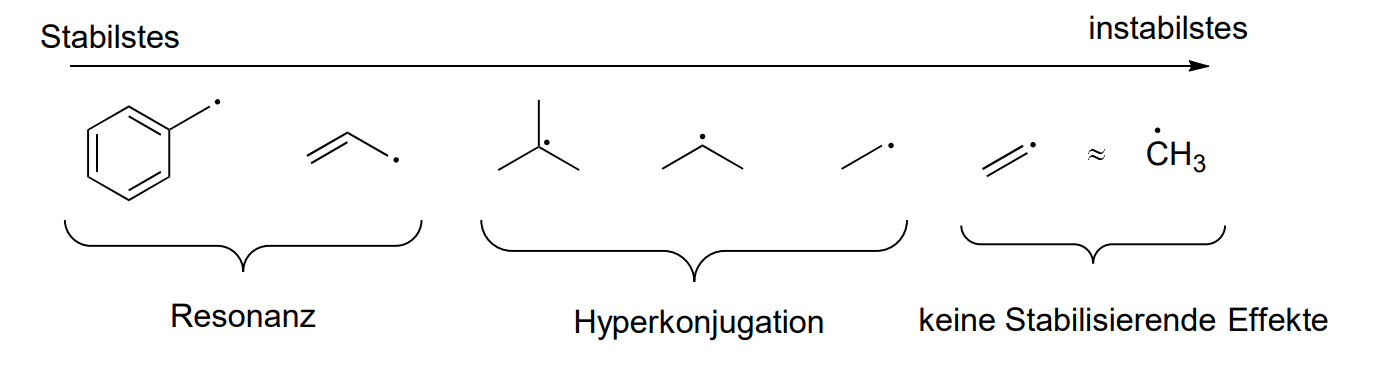
\includegraphics[width=\linewidth]{Bilder/stabilität von Radikalen.png}
\end{figure}

\subsection{Reaktivität von Alkenen vs. Alkine}
Alkene und Alkine weisen annähernd die gleiche Reaktivität auf, jedoch ist das Alkin weniger Nucleophil, als das Alken.

\subsection{Keto-Enol-Tautomerie}
Bei Mechanismen die an Doppelbindungen angreifen um einen Alkohol zu bilden, führt bei Alkinen dazu, dass zuerst das Enol gebildet wird und dieses zügig weiter zum Keton reagiert, da diese Form energetisch günstiger ist.


\subsection{Wagner-Meerwein-Umlagerung}
Die Wagner-Meerwein Umlagerung ist eine Umlagerung einer \ce{CH3}-Gruppe, welche dadurch zu einem stabileren Carbenium-Ion führt.
\begin{figure}[H]
	\centering
	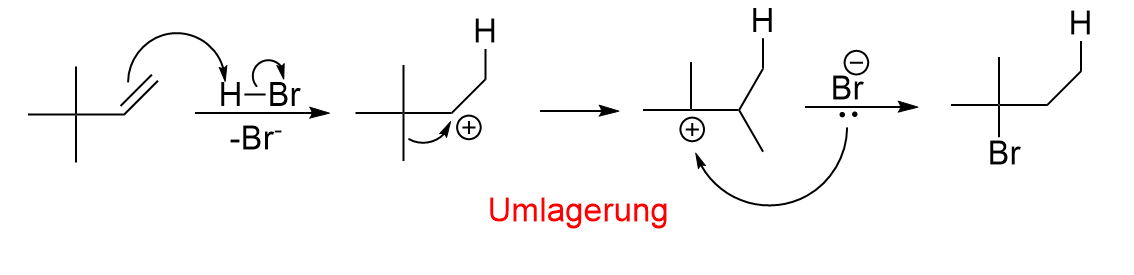
\includegraphics[width=\linewidth]{Bilder/Wagner-Meerwein-Umlagerung.png}
\end{figure}
Wenn eine solche Umlagerung zu einem Stabileren Carbenium-Ion führt, so stellt dieses das Hauptprodukt der Reaktion dar.





\section{Aliphatisch}
\subsection{Radikalische Substitution}
Allgemeiner Mechanismus am Beispiel von Brom.
\begin{figure}[H]
	%\centering
	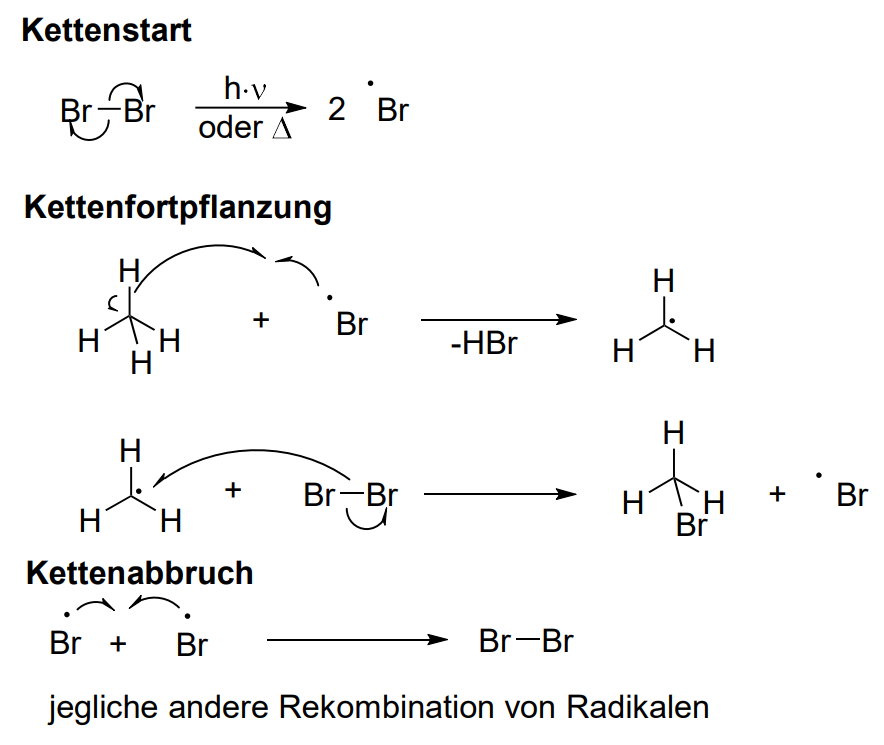
\includegraphics[width=0.7\linewidth]{Bilder/Radikalische Substitution.png}
\end{figure}
\subsubsection{Andere Kettenstartreaktionen}
\subsubsection*{Sulfurylchlorid}
\begin{figure}[H]
	%\centering
	\includegraphics[width=0.7\linewidth]{Bilder/sulfurylchlorid-SR.png}
\end{figure}


\subsubsection{Radikalstarter}
\subsubsection*{Azobis(isobutyronitril) (AIBN)}
\begin{figure}[H]
	\centering
	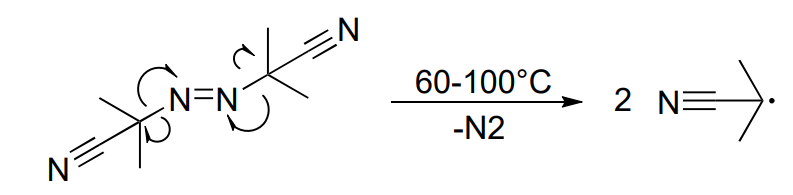
\includegraphics[width=0.6\linewidth]{Bilder/AIBN-Radikalstarter.png}
\end{figure}

\subsubsection*{Dibenzoylperoxid}
\begin{figure}[H]
	\centering
	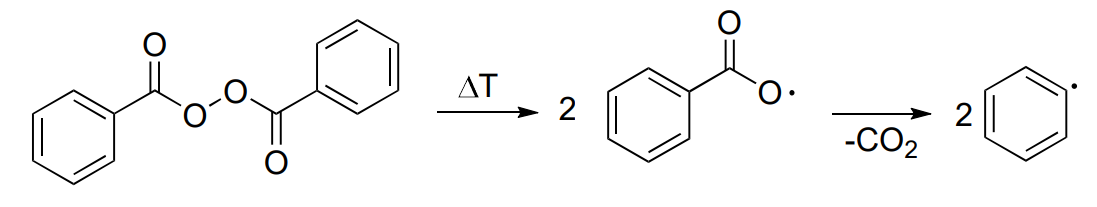
\includegraphics[width=0.7\linewidth]{Bilder/Dibenzoylperoxid-Radikalstarter.png}
\end{figure}

\subsubsection{Radikalische Reduktion}
Die Radikalische Reduktion ist eine Dehalogenierung mit Zinnorganylen.
\subsubsection*{Reaktionsgleichung}
\begin{figure}[H]
	\centering
	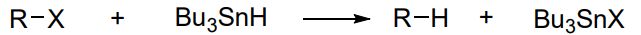
\includegraphics[width=0.55\linewidth]{Bilder/Radikalische Reduktion-Reaktionsgleichung.png}
\end{figure}

\subsubsection*{Mechanismus}
\begin{figure}[H]
	\centering
	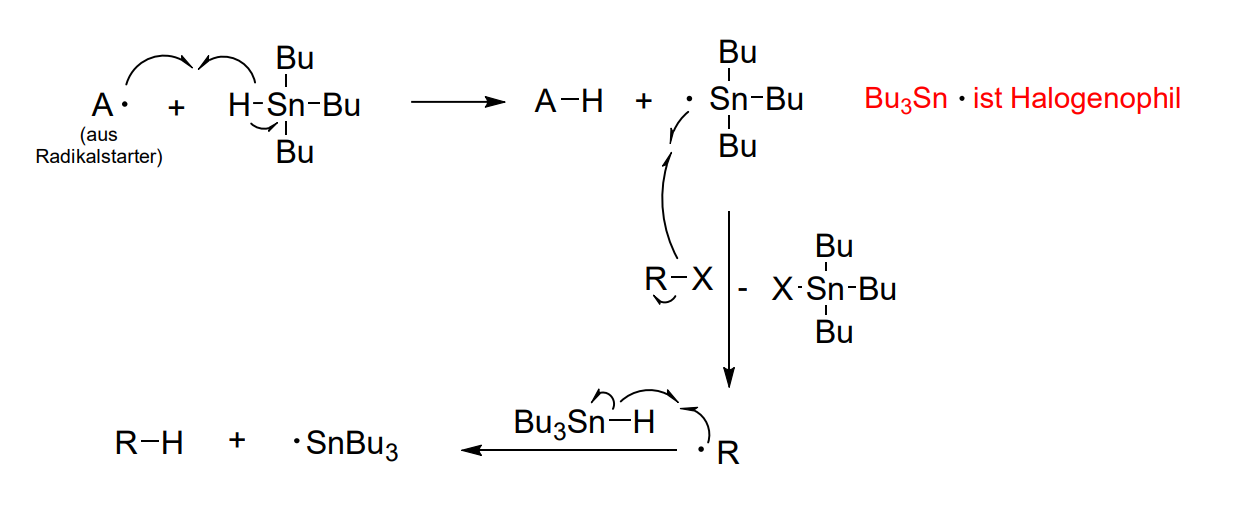
\includegraphics[width=0.85\linewidth]{Bilder/Radikalische Reduktion.png}
\end{figure}


\subsubsection{Radikalische Bromierung mit NBS (Wohl-Ziegler-Bromierung)}
Die Wohl-Ziegler Bromierung nutzt aus, dass Brom nur entsteht, wenn HBr entsteht und so die Radikalische Substitution selektiv ist.
\begin{figure}[H]
	\centering
	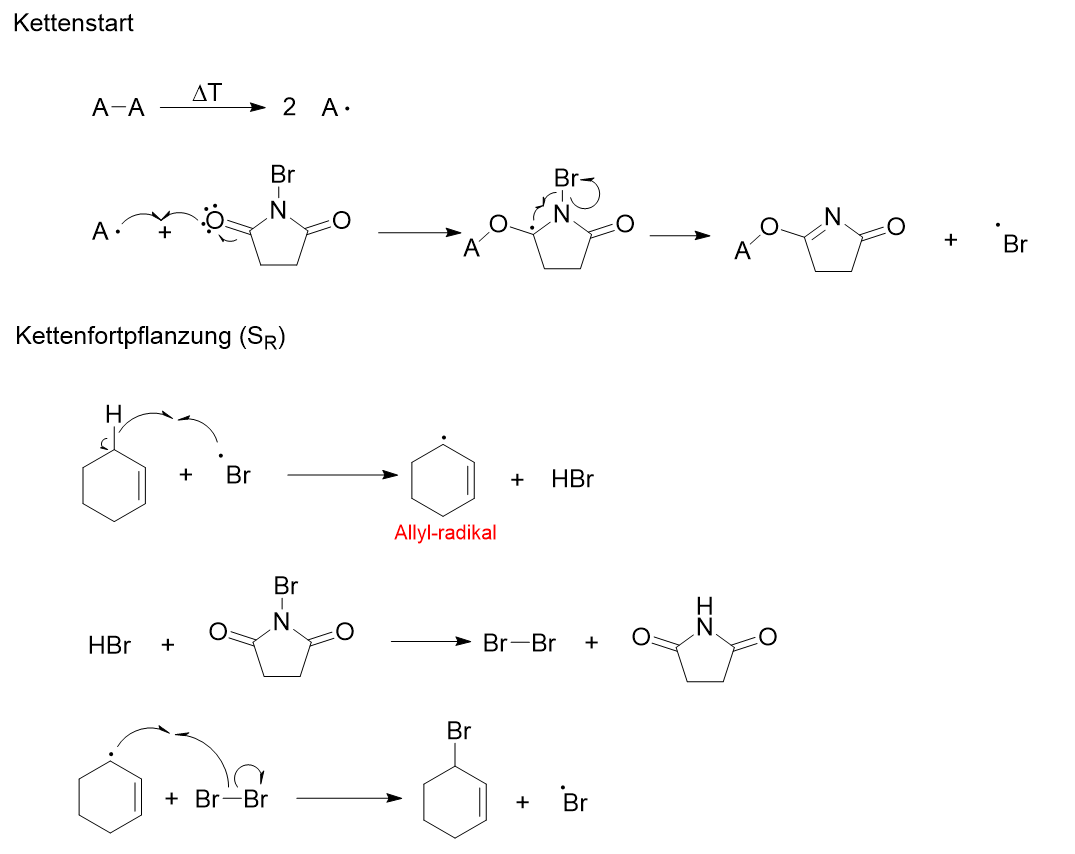
\includegraphics[width=\linewidth]{Bilder/Wohl-Ziegler-Bromierung.png}
\end{figure}


\subsection{Eliminierung}
\subsubsection{Reaktionen}
\begin{figure}[H]
	\centering
	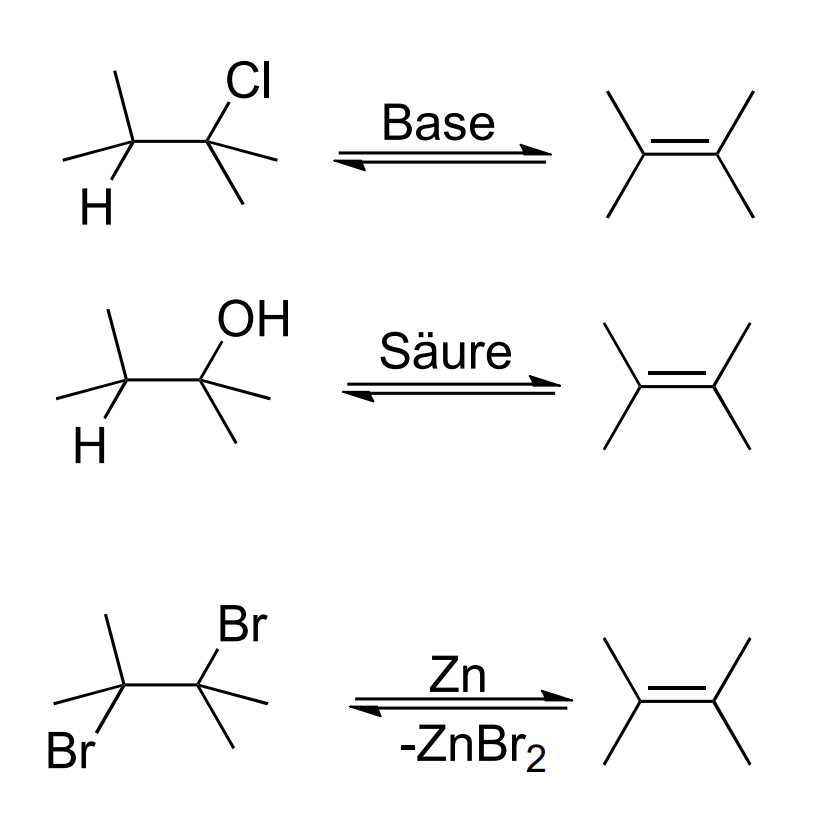
\includegraphics[width=0.4\linewidth]{Bilder/Eliminierungen-Reaktionsgleichungen.png}
\end{figure}


\subsubsection{E2}
\begin{figure}[H]
	\centering
	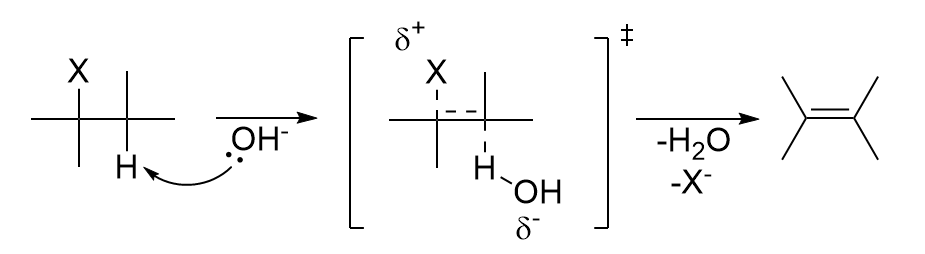
\includegraphics[width=0.8\linewidth]{Bilder/E2.png}
\end{figure}
\ce{E 2}-Eliminierungen weisen eine \textit{trans}-Selektivität auf. Ebenso wird ein höher Substituiertes Alken bevorzugt gebildet (Saytzeff-Regel). Zudem ist die Bildung von konjugierten Alkenen den isolierten bevorzugt.

\subsubsection{E1}
\begin{figure}[H]
	\centering
	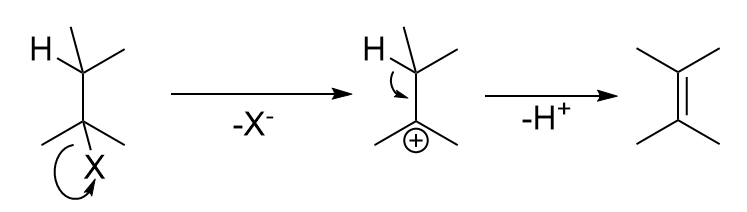
\includegraphics[width=0.7\linewidth]{Bilder/E1-Mechanismus.png}
\end{figure}

\subsubsection{E1cb}
\begin{figure}[H]
	\centering
	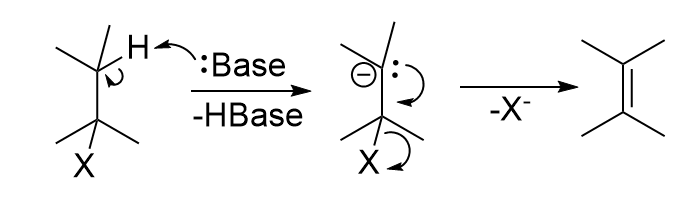
\includegraphics[width=0.7\linewidth]{Bilder/E1cb.png}
\end{figure}
Das abgespaltene Proton muss acide sein und die Base eine starke Base sein. Es werden E-Alkene gebildet.

\subsubsection{Konkurenz E vs \ce{S_N}}
\ce{E 1} und \ce{S_N 1} werden in protisch polaren Lösemitteln stabiliiert. Ist ein Nucleophil eine starke Base und ein schwaches Nucleophil, so ist die Eliminierung bevorzugt. Ist das Nucleophil eine schwache Base und ein gutes Nucleophil, so findet die Substitution statt.
Primäre Halogenalkane machen SN2 und E2, sekundäre Halogenalkane machen SN2, SN1, E2 und E1 und tertiäre Halogenalkane machen SN1, E1, E2. Hohe Temperaturen fördern die Eliminierung.

\subsubsection{Allgemeines zur Eliminierung}
In Cyclischen Verbindungen müssen die zu Eliminierenden Atome in bisaxialer Stellung vorliegen. In Bicyclischen Systemen findet keine Eliminierung zum Brückenkopfatom statt (außer bei Ringen mit mehr als 8-Kohlenstoffen) (Bredtsche Regel).


\subsubsection{Chugaev-Reaktion}
\subsubsection*{Reaktionsgleichung}
\begin{figure}[H]
	\centering
	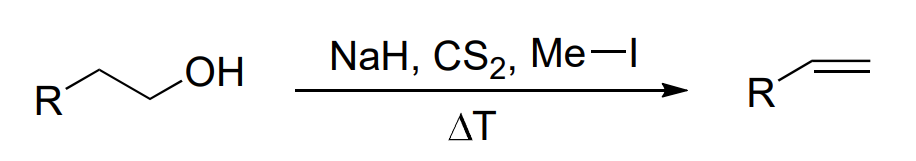
\includegraphics[width=0.6\linewidth]{Bilder/Chugaev-Reaktionsgleichung.png}
\end{figure}


\subsubsection*{Mechanismus}
\begin{figure}[H]
	\centering
	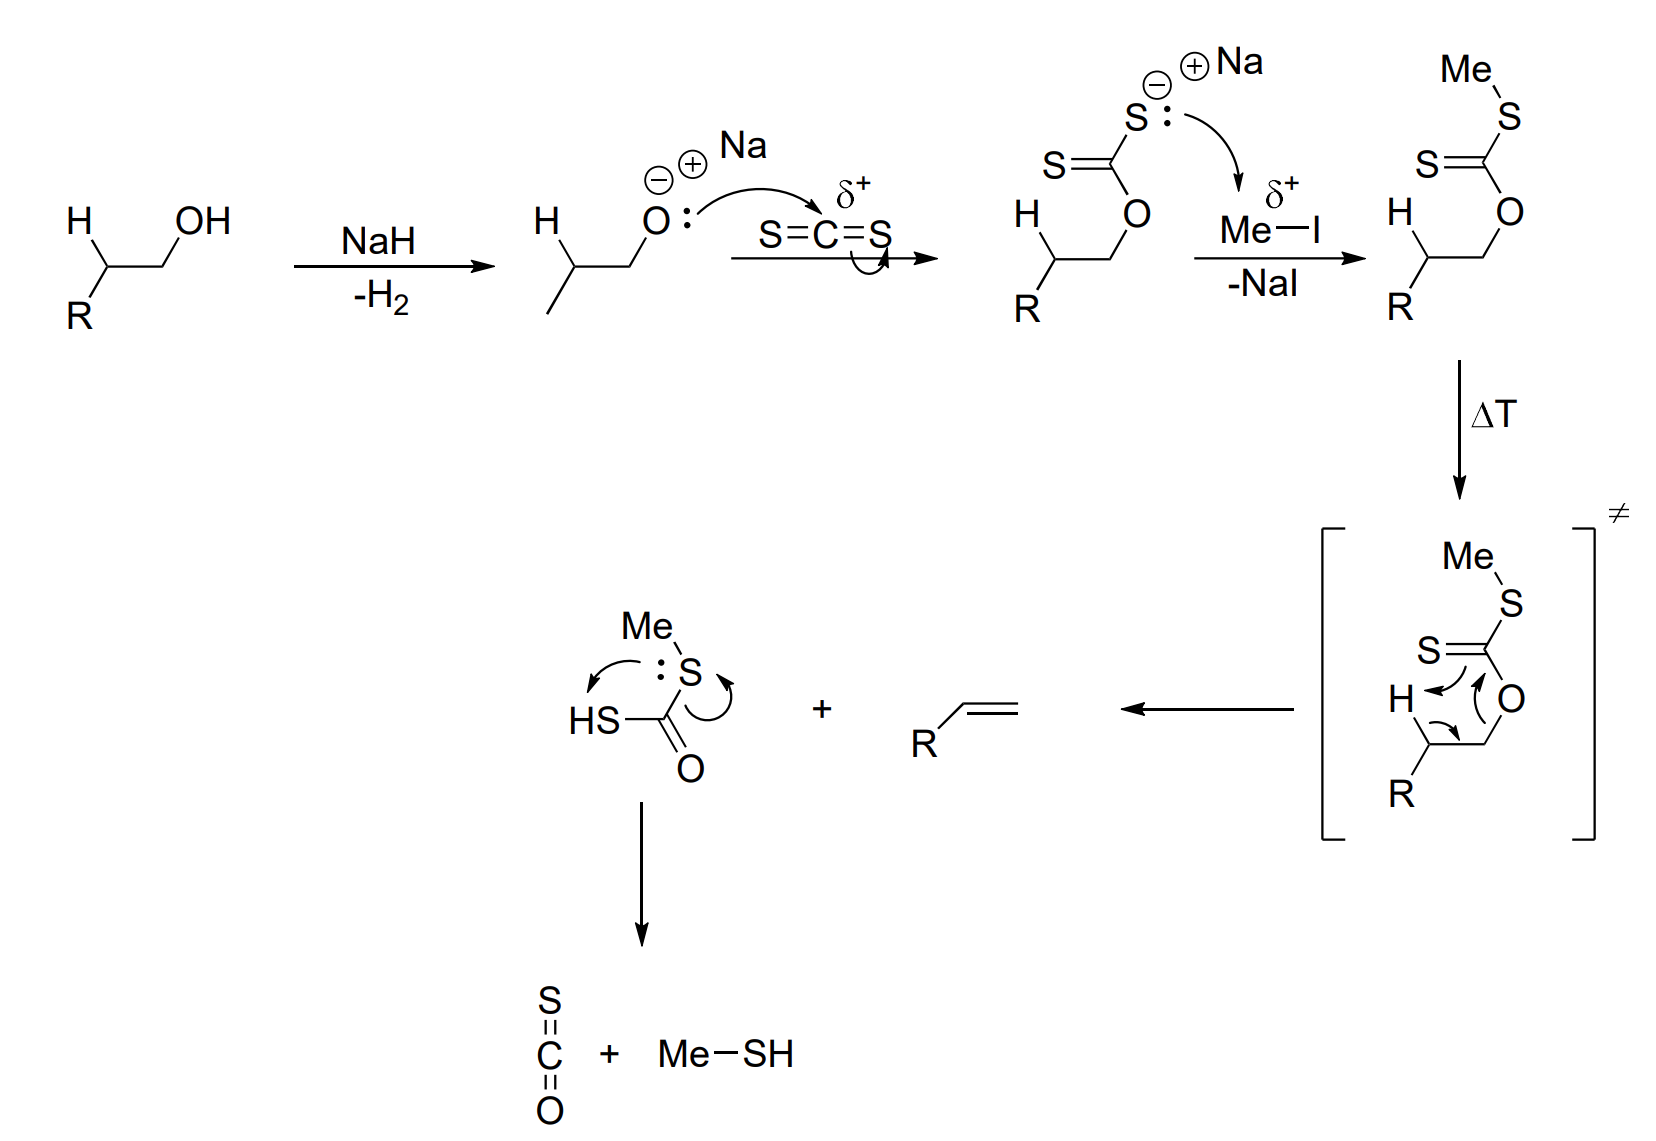
\includegraphics[width=1\linewidth]{Bilder/Chugaev-Mechanismus.png}
\end{figure}


\subsubsection{Esterpyrolyse}
\begin{figure}[H]
	\centering
	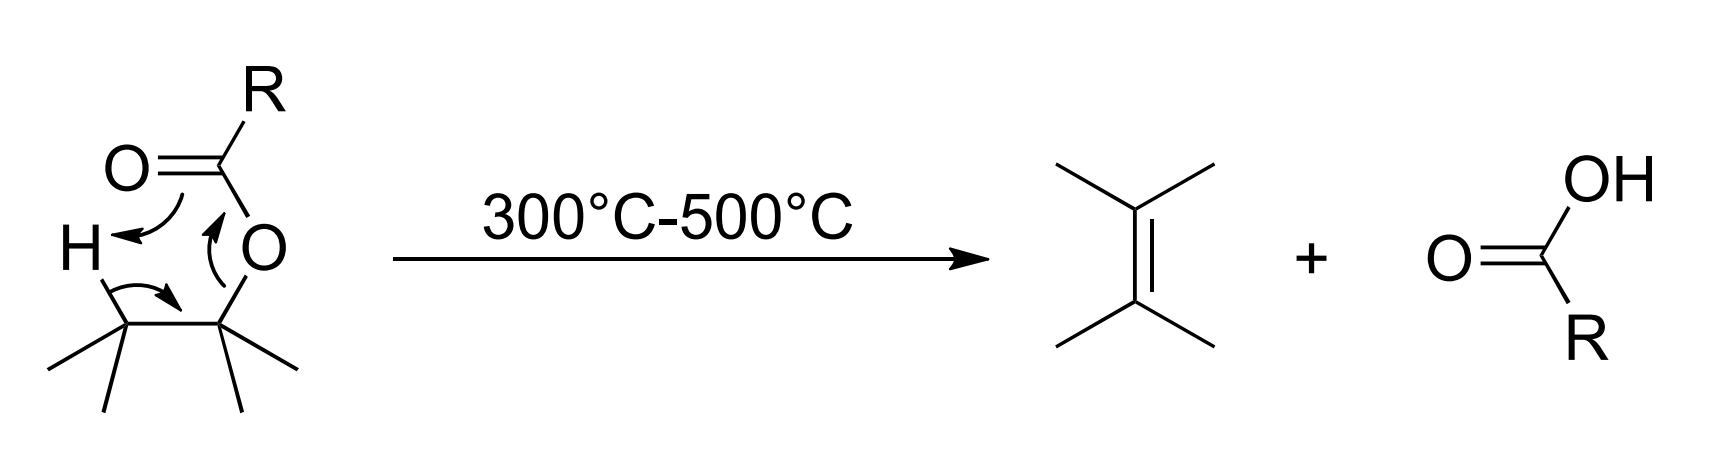
\includegraphics[width=0.7\linewidth]{Bilder/Esterpyrolyse.png}
\end{figure}

\subsubsection{Cope-Eliminierung}
\begin{figure}[H]
	\centering
	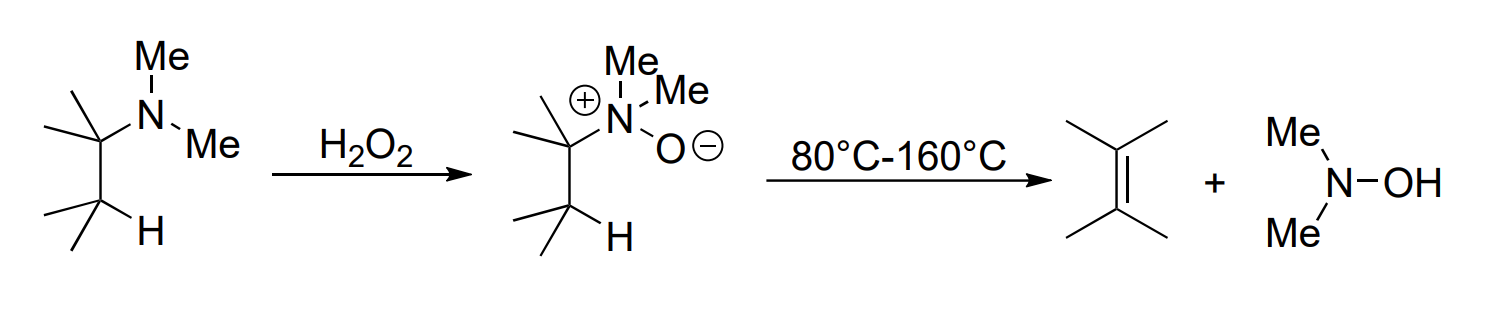
\includegraphics[width=0.95\linewidth]{Bilder/Cope-Eliminierung.png}
\end{figure}






\subsection{Elektrophile Addition}
\subsubsection{Addition von \ce{X2} an Doppelbindungen}
Im Schritt des Carbo-Kations sind mehrere Mesomere möglich. Zum einen gibt es das verbrückte Onium-Ion und das unverbrückte Carbo-Kation. Dies ist abhängig von der Größe des addierten Atoms und der Polarisierbarkeit. Ein großes Atom welches zudem gut polarisierbar ist bildet eher das verbrückte Onium-Ion aus, während andere eher das unverbrückte Carbo-Kation ausbilden. Bei der Addition von Brom bildet sich zum Beispiel das verbrückte Bromonium-Ion. Lediglich die verbrückten Onium-Ionen sind Stereoselektiv, da hier nur der Rückseitenangriff möglich ist und zu einer Anti-Addition führt. Bei einem unverbrückten Carbo-Kation ist die Addition nicht besonders selektiv. Das verbrückte Onium-Ion wird auch als $\sigma$-Komplex bezeichnet.
\begin{figure}[H]
	\centering
	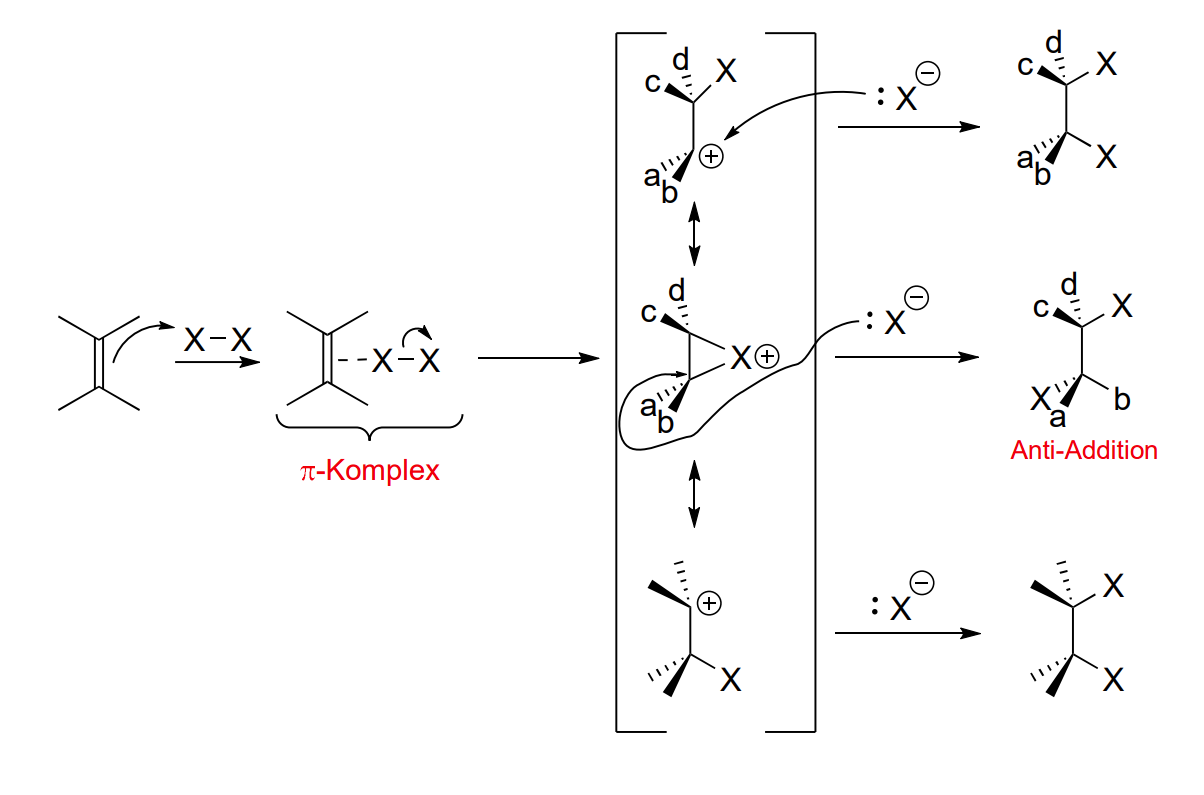
\includegraphics[width=\linewidth]{Bilder/Addition von X2.png}
\end{figure}

\subsubsection{Elektrophile Addition von HX an Doppelbindungen}
\begin{figure}[H]
	\centering
	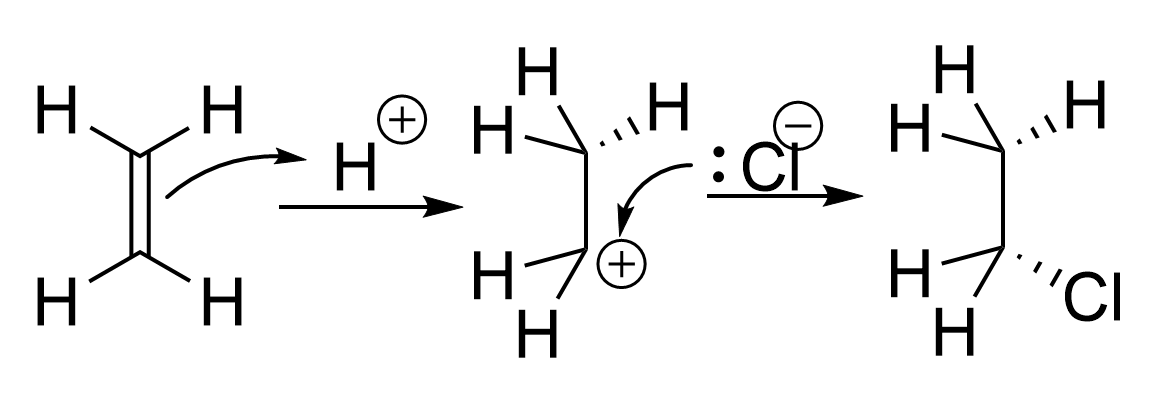
\includegraphics[width=0.55\linewidth]{Bilder/AE-HX an Doppelbindungen.png}
\end{figure}
Diese Addition ist analog zur Addition von \ce{X2} mit unverbrücktem Intermediat, da das Wasserstoff-Atom sehr klein ist.



\subsubsection{Säurekatalysierte Addition von Wasser und Alkoholen}
Bei der Säurekatalysierten Addition von Wasser entsteht ein Alkohol und bei der Addition von Alkoholen entsteht ein Ether.
\begin{figure}[H]
	\centering
	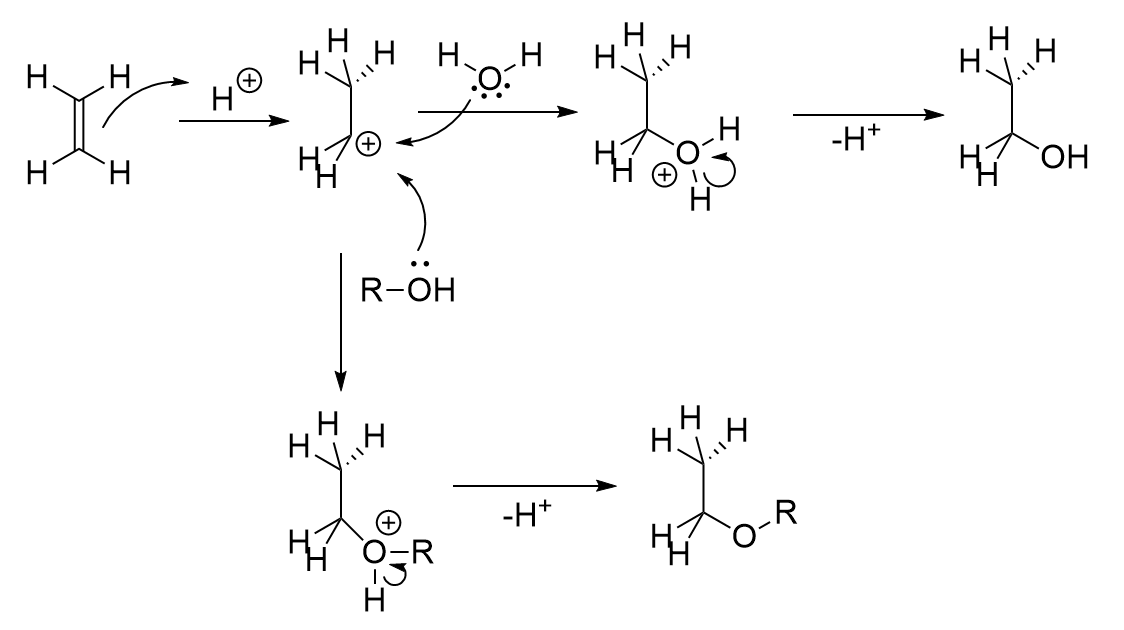
\includegraphics[width=\linewidth]{Bilder/Säurekatalysierte Addition von Wasser und Alkoholen an Doppelbindugnen.png}
\end{figure}

\subsubsection{Addition an konjugierte Doppelbindungen}
\begin{figure}[H]
	\centering
	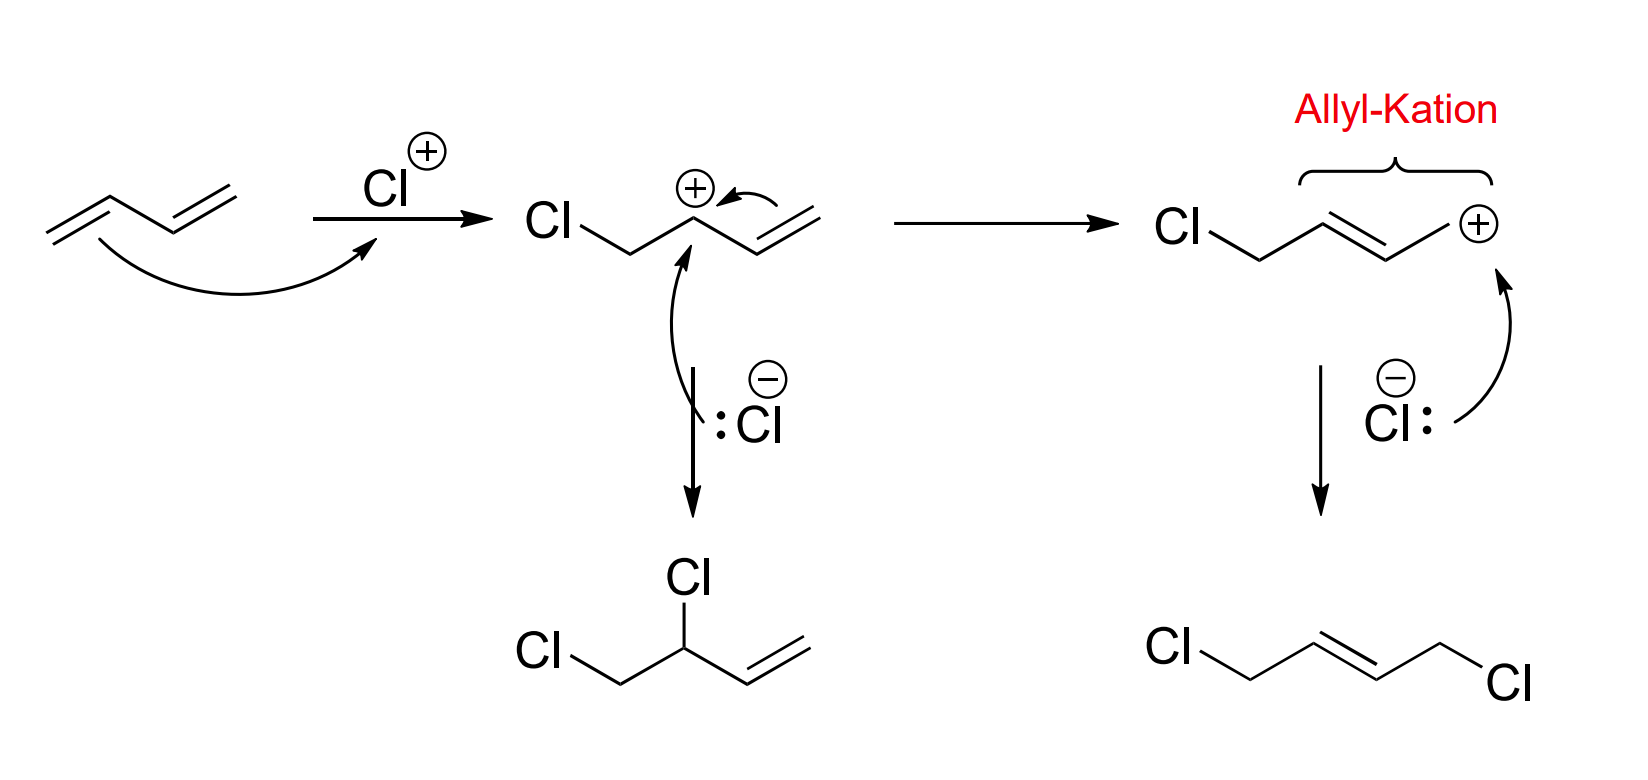
\includegraphics[width=0.85\linewidth]{Bilder/Addition an Konjugierte Doppelbindungen.png}
\end{figure}
Die Struktur des ersten Carbo-Kations ist kein Allyl-Kation, da dieses zwingend endständig sein muss, deshalb ist das zweite Carbo-Kation stabiler da es sich hierbei um das Allyl-Kation handelt.


\subsubsection{Elektrophile Bromierung mit NBS}
\begin{figure}[H]
	\centering
	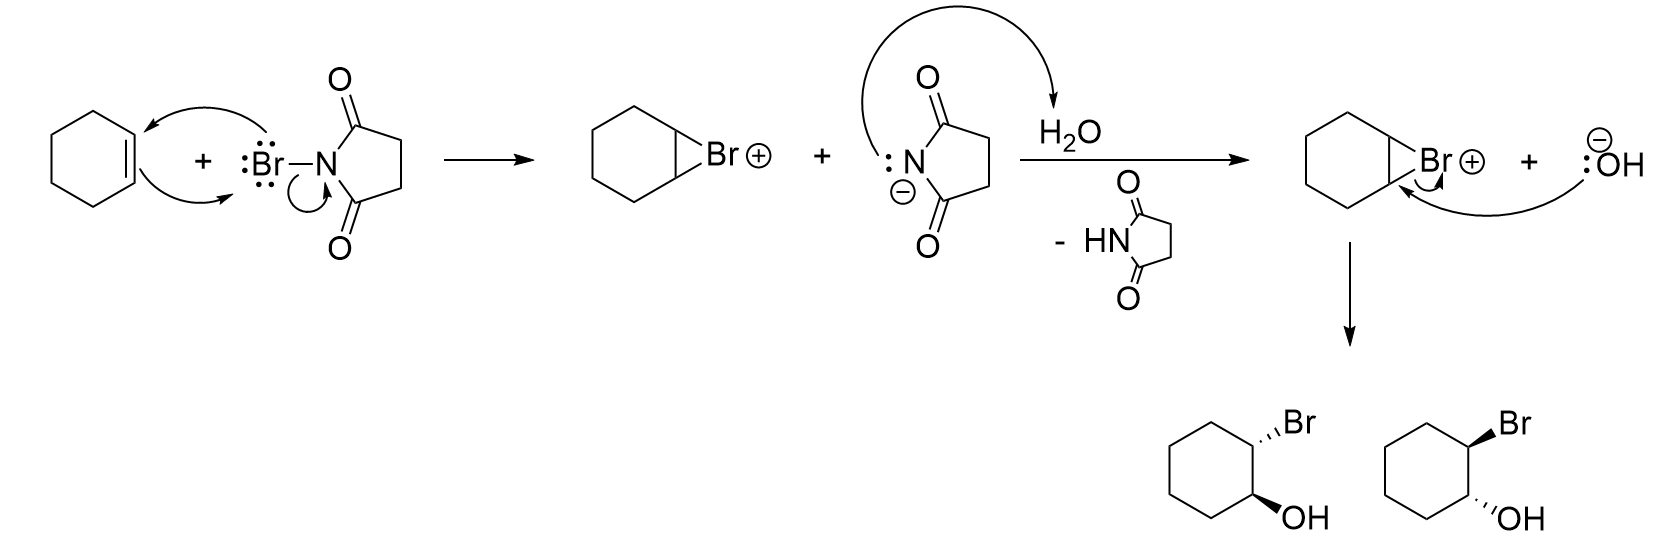
\includegraphics[width=1.1\linewidth]{Bilder/Elektrophile Bromierung mit NBS.png}
\end{figure}

\subsubsection{Oxymercurierung}
\subsubsection*{Reaktionsgleichung}
\begin{figure}[H]
	\centering
	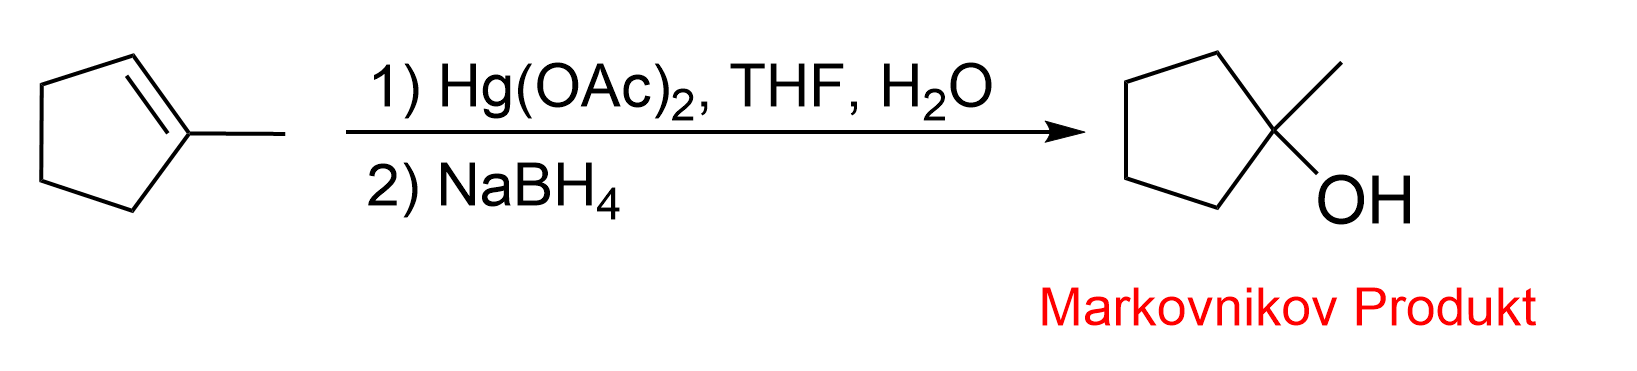
\includegraphics[width=0.8\linewidth]{Bilder/Oxymercurierung-Reaktionsgleichung.png}
\end{figure}

\subsubsection*{Mechanismus}
\begin{figure}[H]
	\centering
	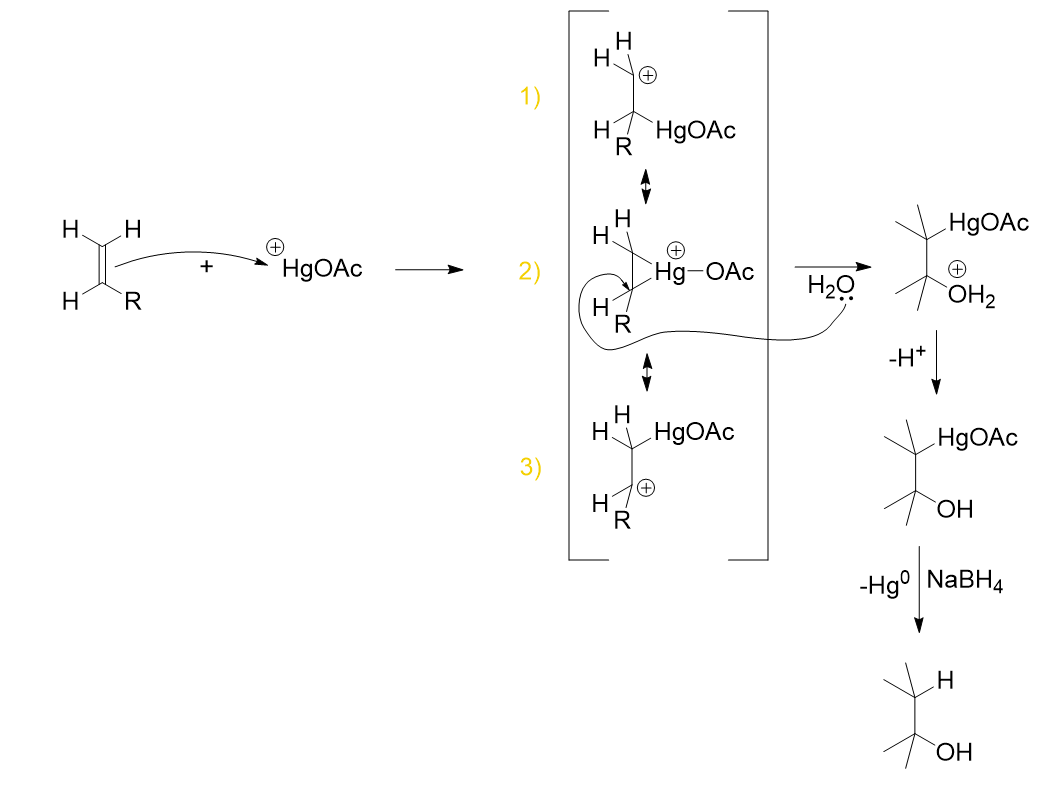
\includegraphics[width=\linewidth]{Bilder/Oxymercurierung-Mechanismus.png}
\end{figure}
Von den Mesomeren Grenzstrukturen ist 2) am warscheinlichsten, 3) immernoch warscheinlich und 1) unwarscheinlich. Dies liegt, daran, dass der Alkylrest für ein Sekundäres Carbo-Kation sorgt und dieses stabiler ist, wie am Kohlenstoff mit lediglich zwei Wasserstoff-Atomen.


\subsubsection{Hydroborierung}
\subsubsection*{Reaktionsgleichung}
\begin{figure}[H]
	\centering
	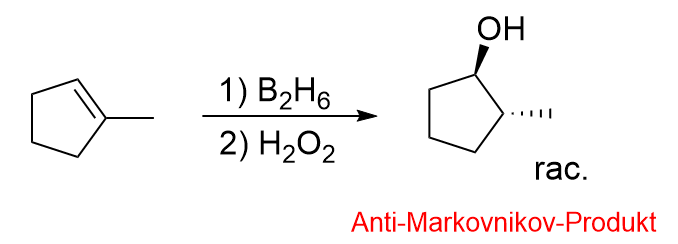
\includegraphics[width=0.55\linewidth]{Bilder/Hydroborierung-Reaktionsgleichung.png}
\end{figure}

\subsubsection*{Mechanismus}
\begin{figure}[H]
	\centering
	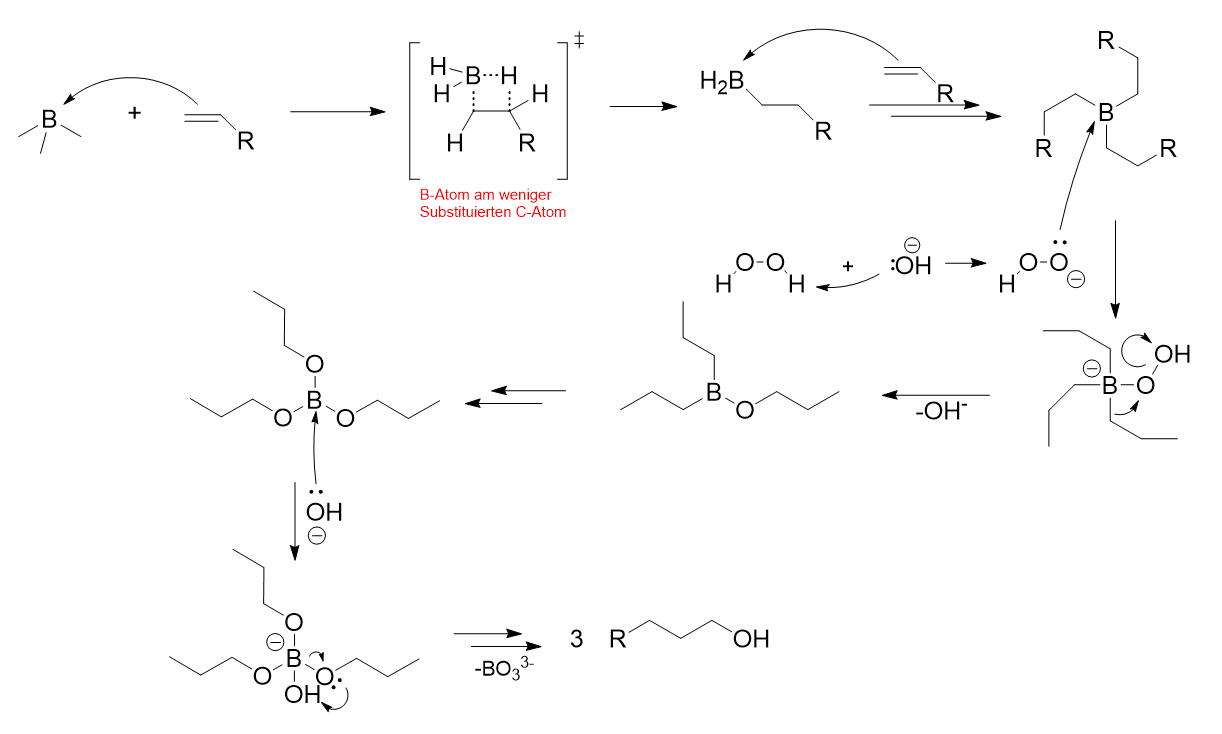
\includegraphics[width=\linewidth]{Bilder/Hydroborierung-Mechanismus.png}
\end{figure}




\subsubsection{Epoxidierung von Doppelbindungen}
\subsubsection*{Reaktionsgleichung}
\begin{figure}[H]
	\centering
	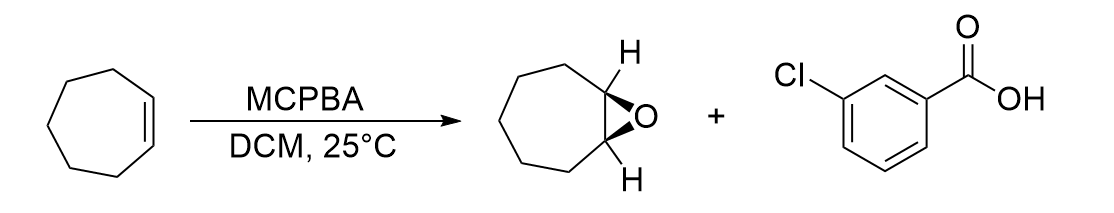
\includegraphics[width=0.8\linewidth]{Bilder/Epoxidierung-Reaktionsgleichung.png}
\end{figure}
Wobei MCPBA (m-Chlorperbenzoesäure) wie folgt aussieht
\begin{figure}[H]
	\centering
	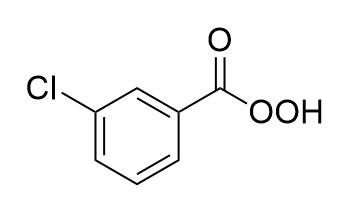
\includegraphics[width=0.3\linewidth]{Bilder/MCPBA-Strukturformel.png}
\end{figure}

\subsubsection*{Mechanismus}
\begin{figure}[H]
	\centering
	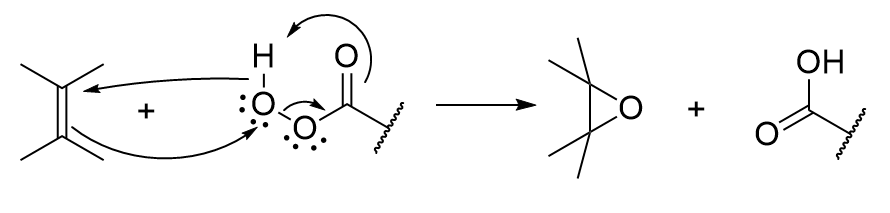
\includegraphics[width=0.75\linewidth]{Bilder/Epoxidierung-Mechanismus.png}
\end{figure}
\subsubsection*{Aufarbeitung}
\begin{figure}[H]
	\centering
	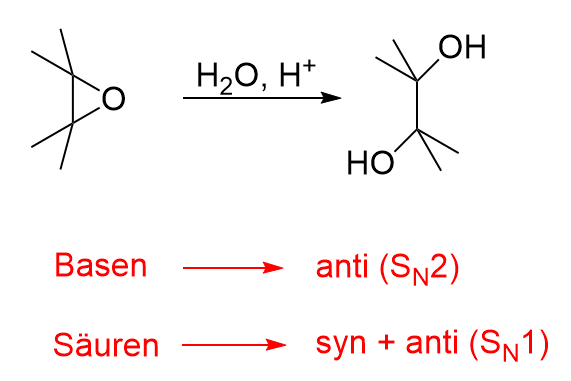
\includegraphics[width=0.5\linewidth]{Bilder/Epoxidierung-Aufarbeitung.png}
\end{figure}
Bei der Aufarbeitung im basischen entscheidet die Sterik, auf welcher Seite des Epoxid-Kohlenstoffs das Nucleophil angreift. Es greift dort am sterisch weniger gehinderten Kohlenstoff an. Im Sauren ist das Sauerstoff des Epoxid-Rings protoniert und liegt ein verbrücktes Hydroxid vor, welches am sterisch mehr gehinderten Kohlenstoff positiver ist, wie am sterisch weniger gehinderten, aufgrund der stabilisierenden Effekte von Alkylresten. Somit greift das Nukleophil im sauren am sterisch mehr gehinderten Kohlenstoff-Atom des Epoxids an.

\subsubsection*{Metallkatalysierte Epoxidierung}
\begin{figure}[H]
	\centering
	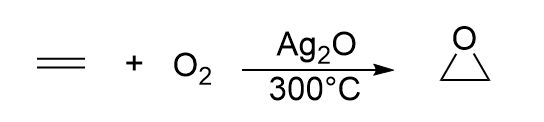
\includegraphics[width=0.5\linewidth]{Bilder/Metallkatalysierte-Epoxidierung.png}
\end{figure}

\subsubsection*{Aus Halogenhydrinen}
\begin{figure}[H]
	\centering
	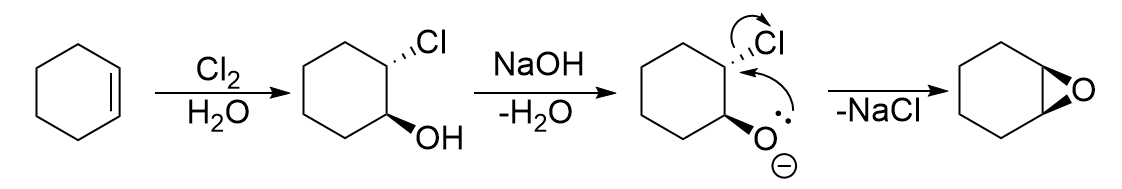
\includegraphics[width=\linewidth]{Bilder/Halogenhydrinen-epoxidierung.png}
\end{figure}



\subsection{Radikalische Addition}
\subsubsection{Radikalische Addition an Doppelbindungen}
\begin{figure}[H]
	\centering
	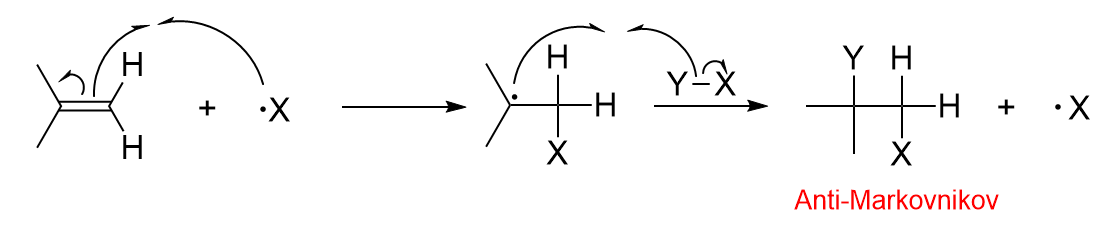
\includegraphics[width=0.9\linewidth]{Bilder/AR-Alkene.png}
\end{figure}



\subsubsection{Radikalische Alkylierung von Doppelbindungen}
\subsubsection*{Reaktionsgleichung}
\begin{figure}[H]
	\centering
	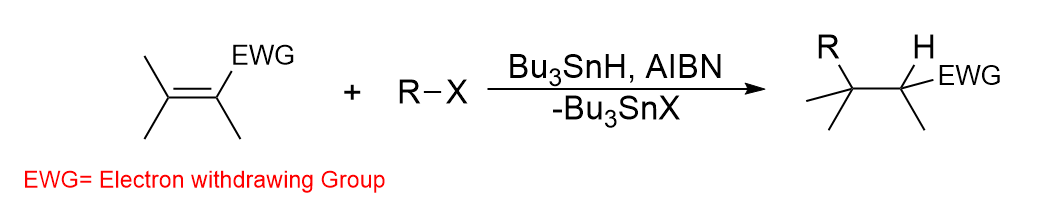
\includegraphics[width=0.9\linewidth]{Bilder/Radikalische Alkylierung-Reaktionsgleichung.png}
\end{figure}

\subsubsection*{Mechanismus}
\begin{figure}[H]
	\centering
	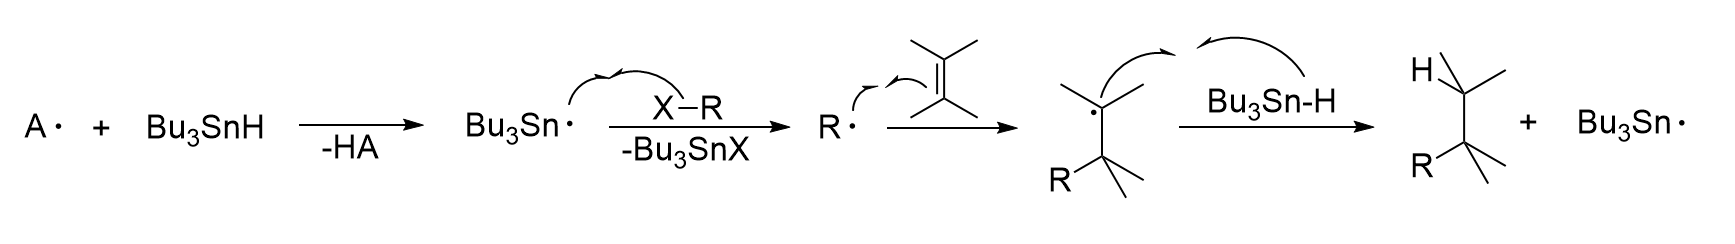
\includegraphics[width=1.2\linewidth]{Bilder/Radikalische Alkylierung-Mechanismus.png}
\end{figure}



\subsection{Cycloaddition}
\subsubsection{Diels-Alder ([4+2]-Cycloaddition)}
\begin{figure}[H]
	\centering
	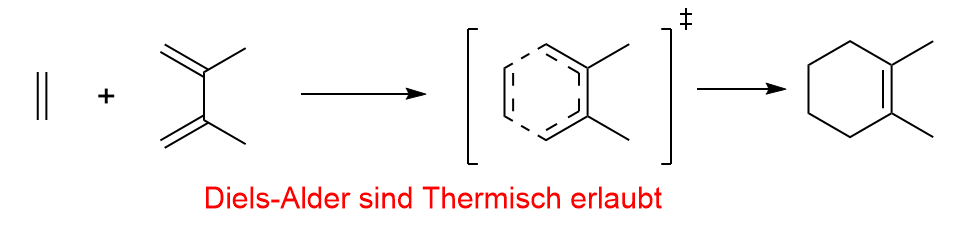
\includegraphics[width=0.9\linewidth]{Bilder/Diels-Alder.png}
\end{figure}


\subsubsection{Criegee Oxidation (Ozonolyse)}
\subsubsection*{Mechanismus}
\begin{figure}[H]
	\centering
	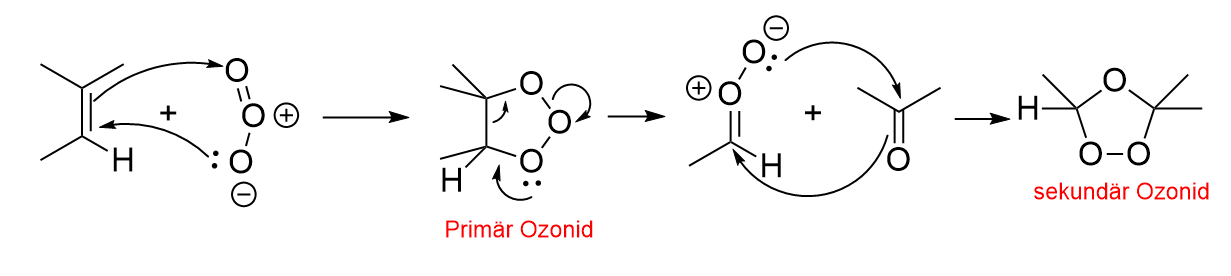
\includegraphics[width=\linewidth]{Bilder/Ozonolyse-Mechanismus.png}
\end{figure}

\subsubsection*{Aufarbeitung}
\begin{figure}[H]
	\centering
	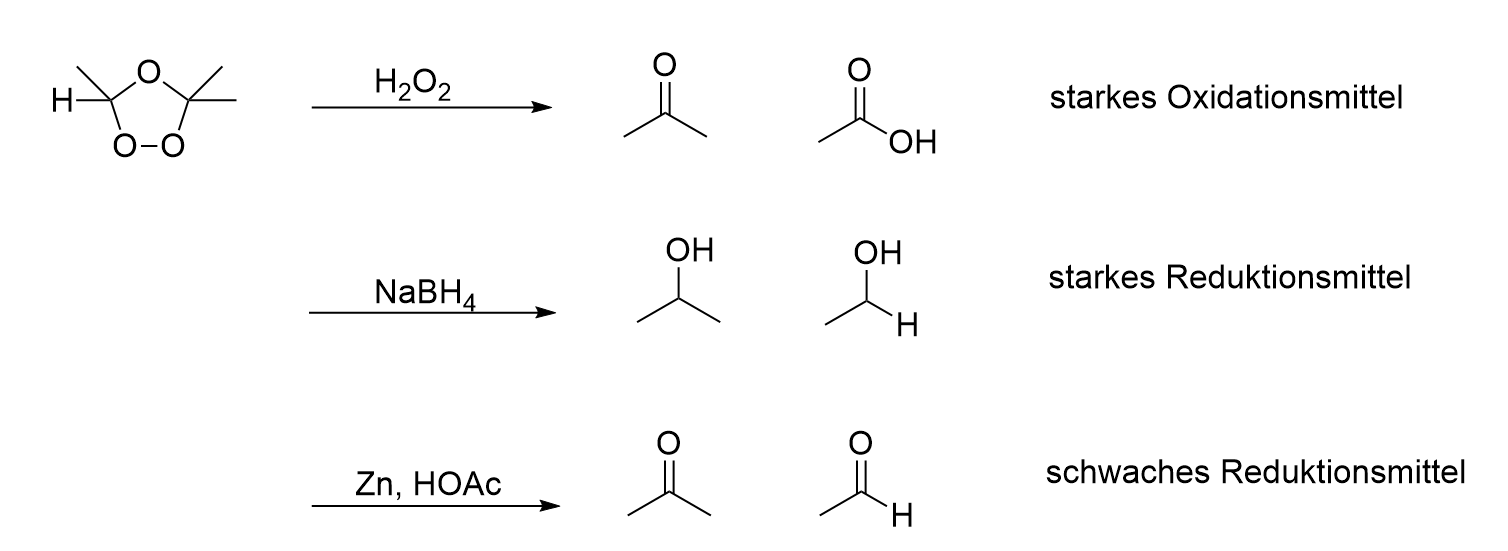
\includegraphics[width=\linewidth]{Bilder/Ozonolyse-Aufarbeitung.png}
\end{figure}

\subsubsection{Oxidation mit \ce{KMnO4}}
\begin{figure}[H]
	\centering
	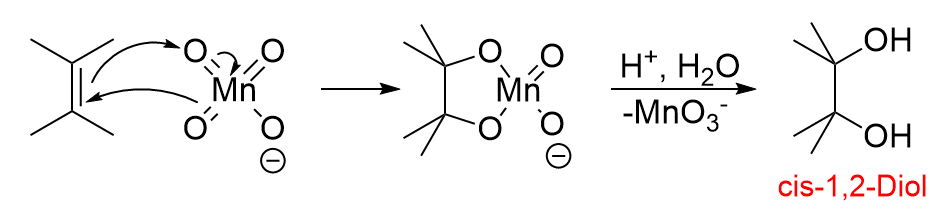
\includegraphics[width=0.85\linewidth]{Bilder/Oxidation mit KMnO4.png}
\end{figure}

\subsubsection{Oxidation mit \ce{OsO4}}
\begin{figure}[H]
	\centering
	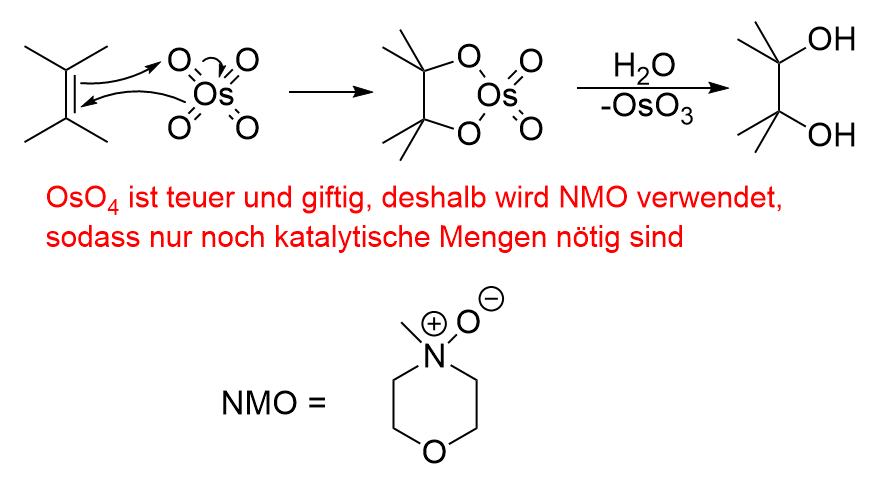
\includegraphics[width=0.7\linewidth]{Bilder/Oxidation mit OsO4.png}
\end{figure}


\subsection{Nucleophile Substitution}
\subsubsection{\ce{S_N 2}}
\begin{figure}[H]
	\centering
	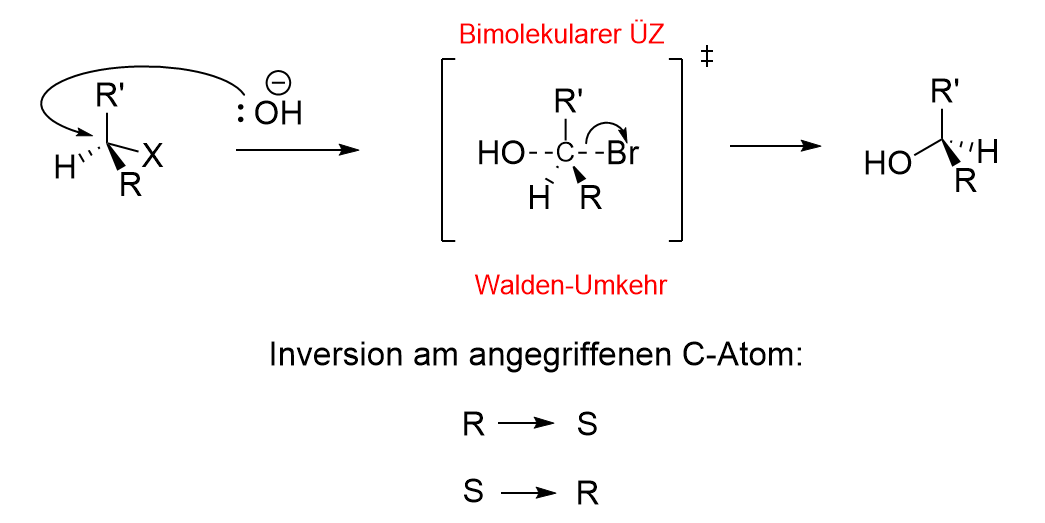
\includegraphics[width=0.95\linewidth]{Bilder/SN1.png}
\end{figure}
\noindent Der \ce{S_N 2} Mechanismus läuft bei primär und sekundären Kohlenstoffen ab, bei tertiären ist dieser nicht möglich. Der Geschwindigkeitsbestimmende Reaktionsschritt ist Bimolekular, weshalb die Reaktion mit einer 2 bezeichnet wird. Sie finden in polar aprotischen Lösemitteln statt. Die Substitution steht in Konkurenz zur E2 Reaktion.

\subsubsection{\ce{S_N 1}}
Der Geschwindigkeitsbestimmende Schritt ist Monomolekular, was mit einer 1 gekennzeichnet wird. Sie finden in Protischen Lösemitteln statt. Die Substitution steht in Konkurenz zur E1 Reaktion.
\begin{figure}[H]
	\centering
	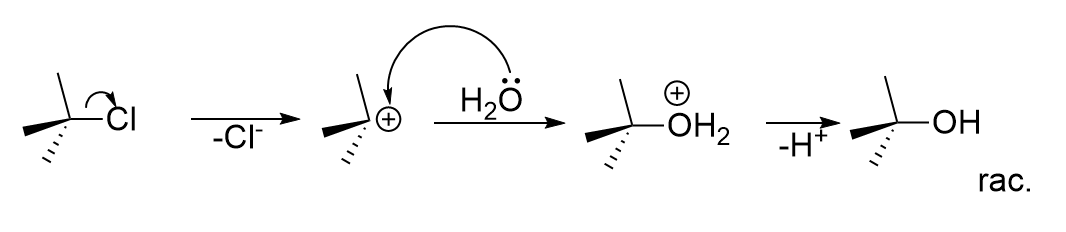
\includegraphics[width=\linewidth]{Bilder/SN2.png}
\end{figure}
\noindent Am Carbenium-Ion kann eine Wagner-Meerwein-Umlagerung stattfinden.\\

\noindent Um zu verhindern, dass ein Racemat entsteht kann folgende Reaktion verwendet werden.
\begin{figure}[H]
	\centering
	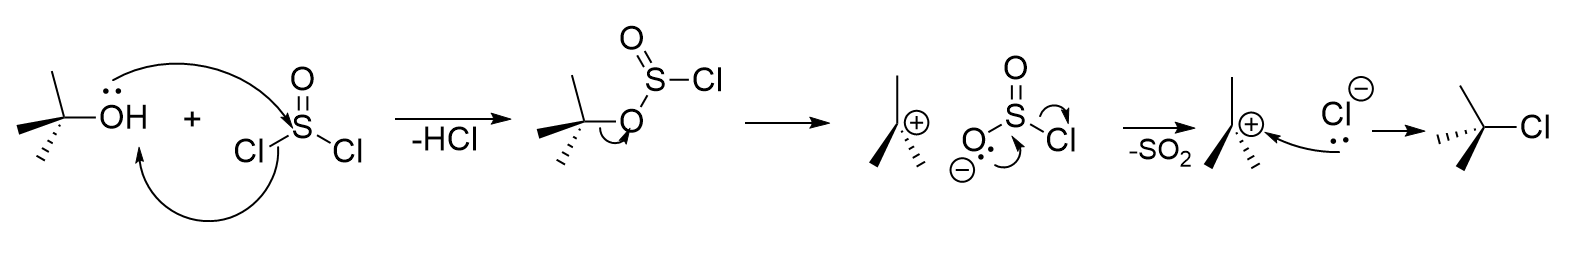
\includegraphics[width=1.1\linewidth]{Bilder/SN1 mit SOCl2.png}
\end{figure}

\subsubsection{Finkelstein-Reaktion}
Die Finkelstein ist eine Umhalogenierung nach SN2 Mechanismus. 
Eingesetzt wird ein Natriumhalogenid Salz und als Lösemittel ein aprotisch polares. Die Löslichkeit der Natriumhalogenide in Aceton nimmt mit steigender Ordnungszahl des Halogenids, aufgrund ihrer polarisierbarkeit zu. Somit kann zum Beispiel ein Chlor-Substituent mit einem Iodid getauscht werden, da Natriumiodid in Aceton relativ gut löslich ist, Natriumchlorid aber nicht und damit ausfällt. Dies ist die Triebkraft der Finkelstein-Reaktion.
\begin{figure}[H]
	\centering
	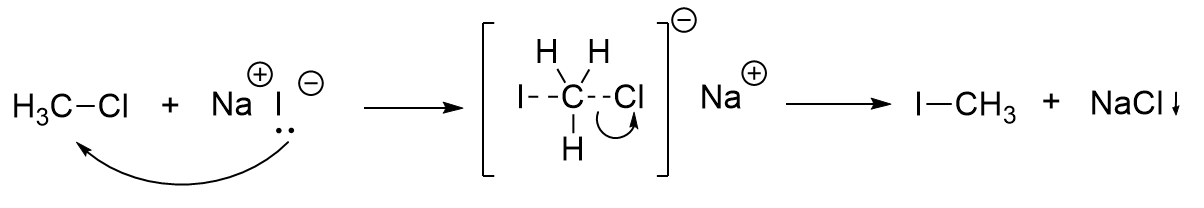
\includegraphics[width=\linewidth]{Bilder/Finkelstein.png}
\end{figure}
\noindent Bei primären Alkylhalogeniden findet die Reaktion schnell und mit hohen Ausbeuten statt, bei sekundären langsamer und nur noch moderate Ausbeuten und bei tertären findet keine Reaktion statt.

\subsubsection{Gabriel-Synthese}
\begin{figure}[H]
	\centering
	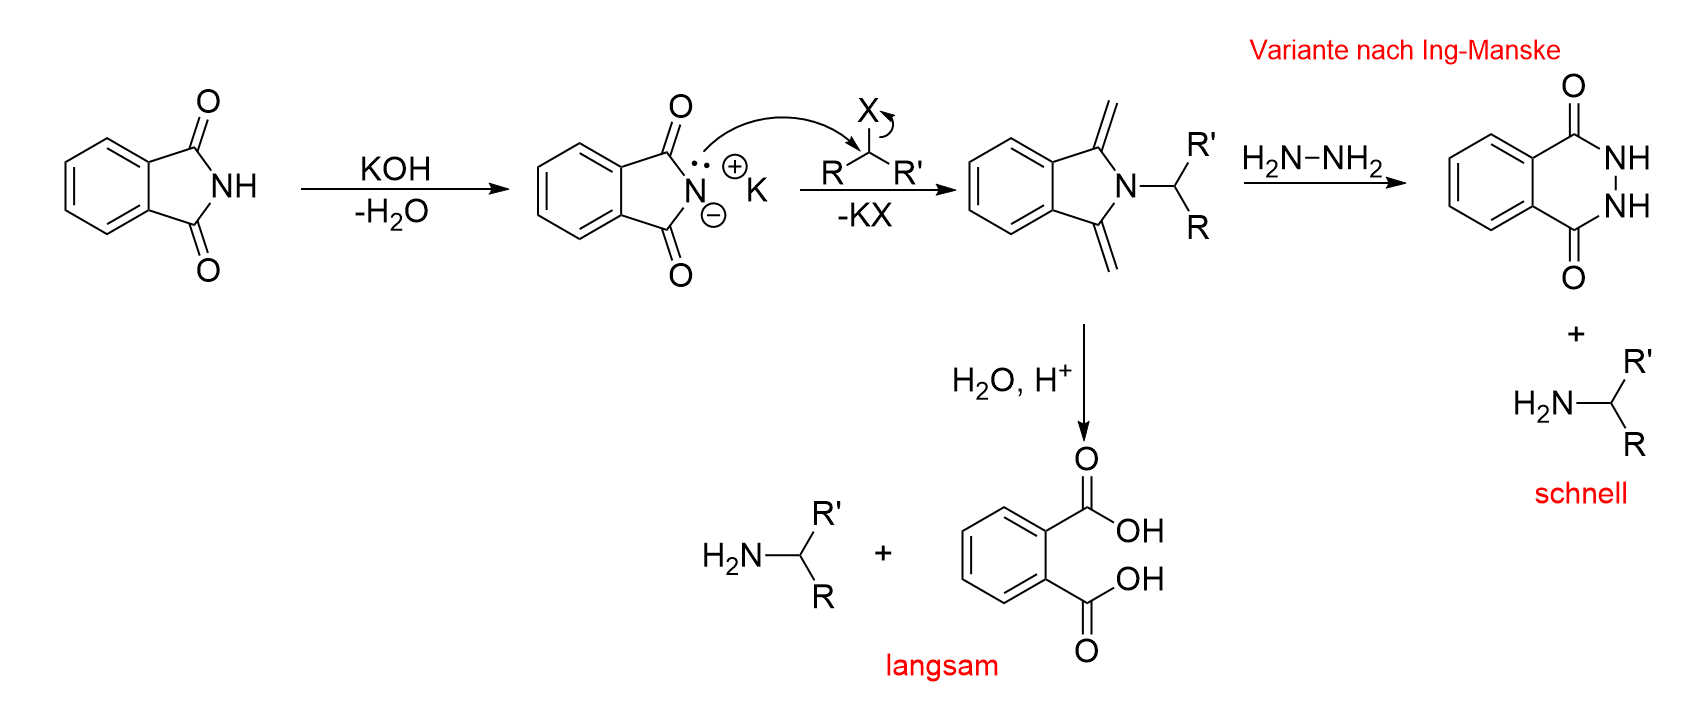
\includegraphics[width=1.1\linewidth]{Bilder/Gabriel-Synthese.png}
\end{figure}

\subsubsection{Alkylierung von Phosphorverbindungen}
\begin{figure}[H]
	\centering
	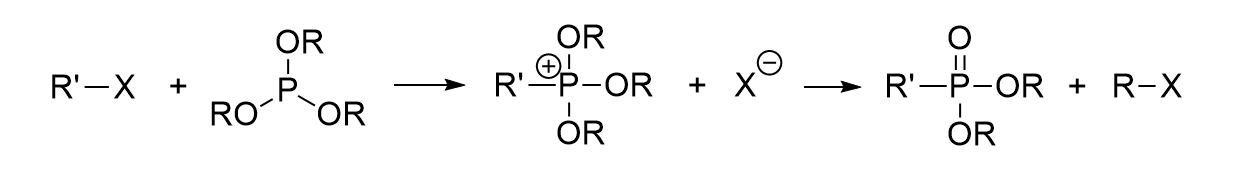
\includegraphics[width=\linewidth]{Bilder/Alkylierung von Phosphorverbindungen.png}
\end{figure}

\subsubsection{Kolbe Nitrilsynthese}
\begin{figure}[H]
	\centering
	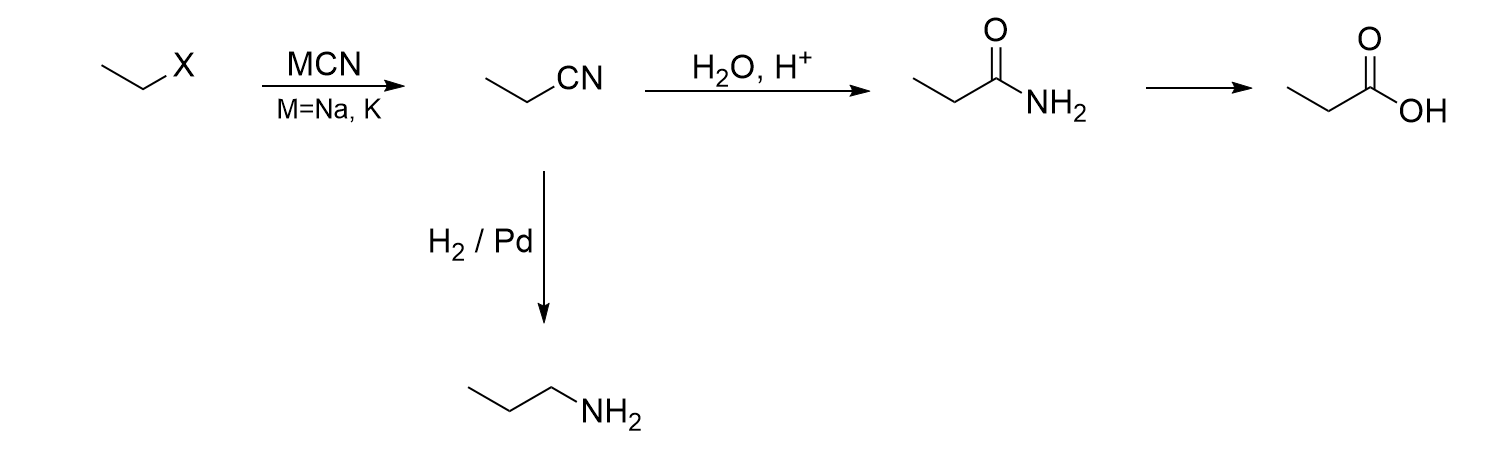
\includegraphics[width=\linewidth]{Bilder/Kolbe Nitrilsynthese.png}
\end{figure}
Die Kolbe-Nitrilsynthese ist eine typische SN2 Reaktion. 
Aprotische Lösemittel wie Aceton oder DMSO sind günstig, bei primären Alkylhalogeniden findet die Reaktion schnell mit hohen
Ausbeuten statt, bei sekundären, langsamer und moderaten Ausbeuten und bei tertiären keine Reaktion, lediglich eine langsame Eliminierung.

\subsubsection{Appel-Reaktion}
\subsubsection*{Reaktionsgleichung}
\begin{figure}[H]
	\centering
	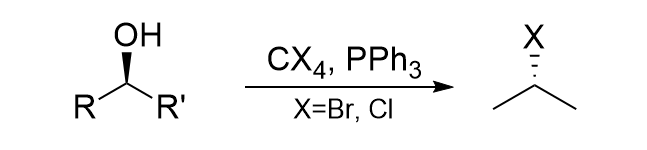
\includegraphics[width=0.6\linewidth]{Bilder/Appel-Reaktionsgleichung.png}
\end{figure}
\subsubsection*{Mechanismus}
\begin{figure}[H]
	\centering
	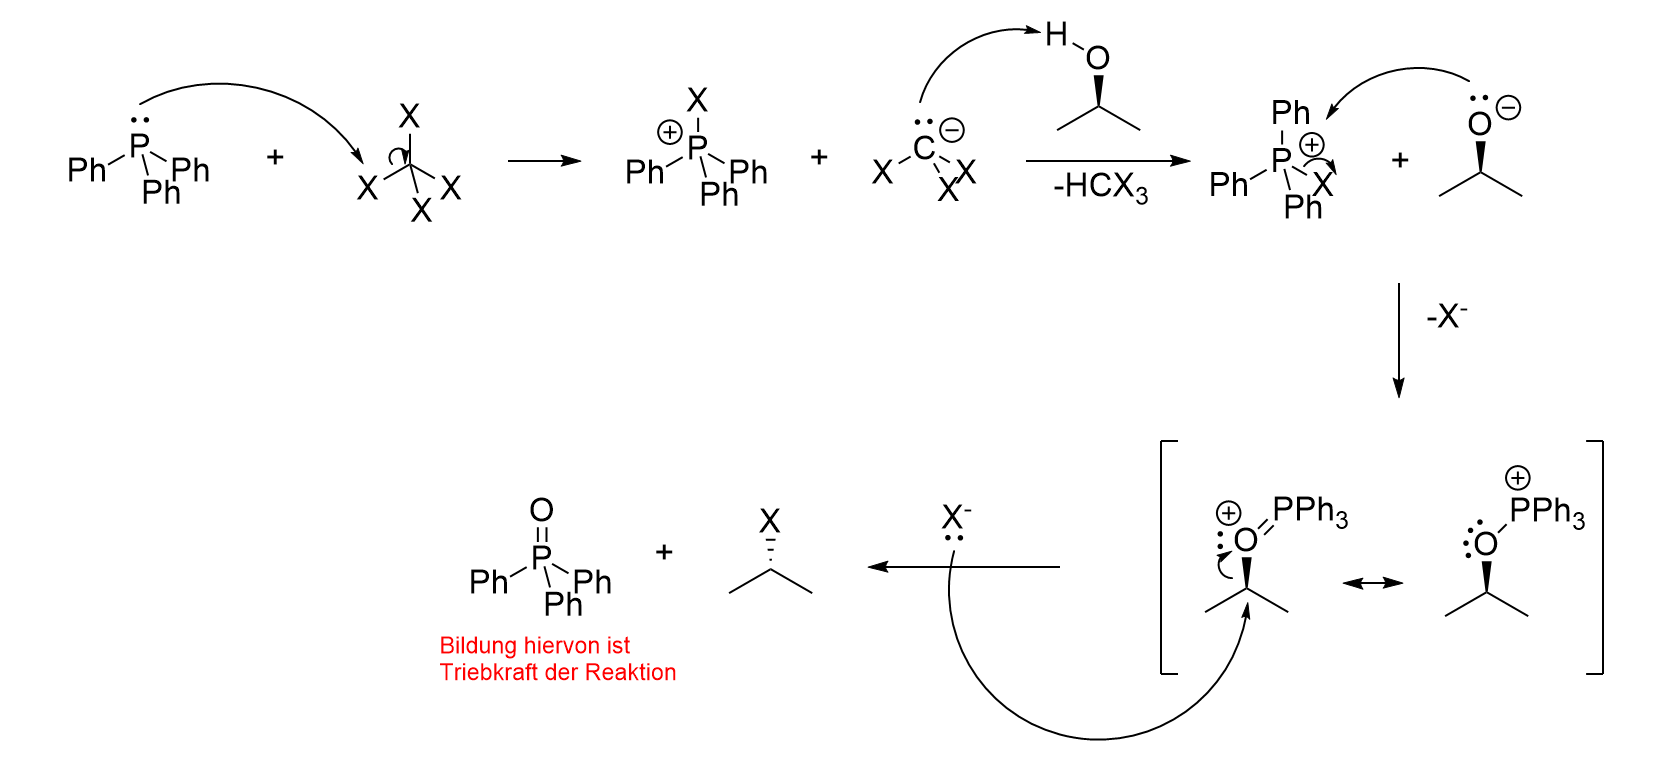
\includegraphics[width=1.1\linewidth]{Bilder/Appel-Reaktion.png}
\end{figure}

\subsubsection{Darstellung von Thiolen mit Thioharnstoff}
\begin{figure}[H]
	\centering
	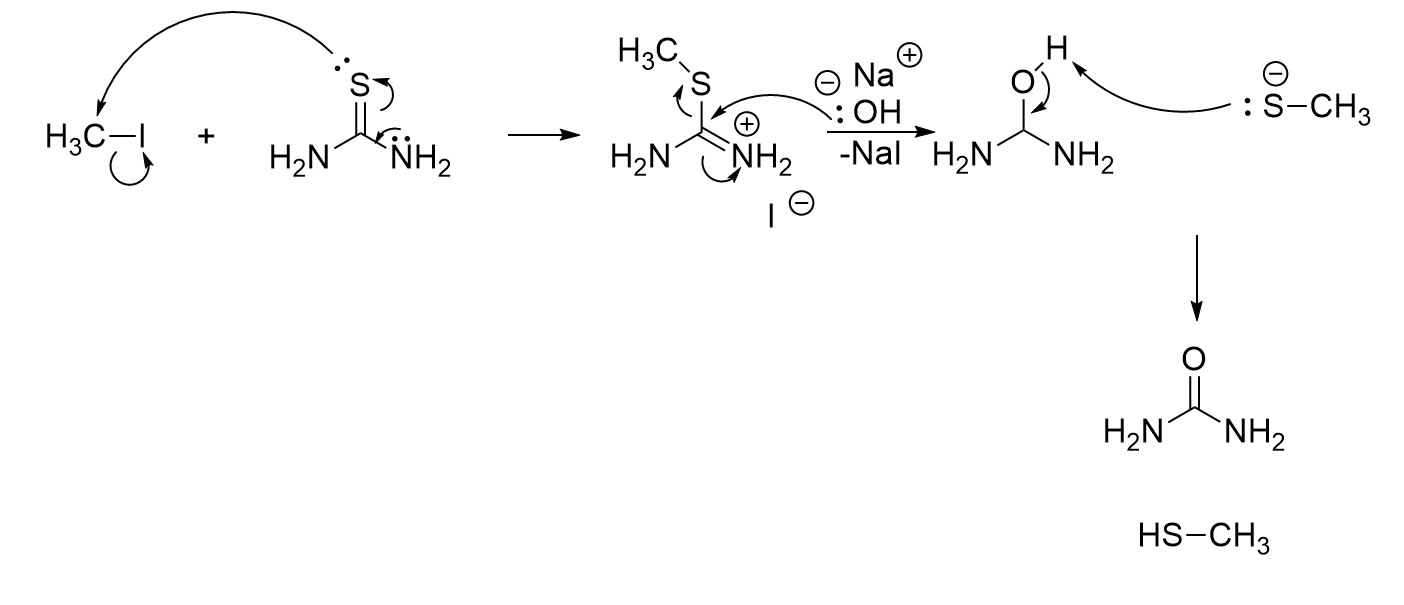
\includegraphics[width=\linewidth]{Bilder/Thiole aus Thioharnstoff.png}
\end{figure}


\subsubsection{Williamsonsche Ethersynthese}
\begin{figure}[H]
	\centering
	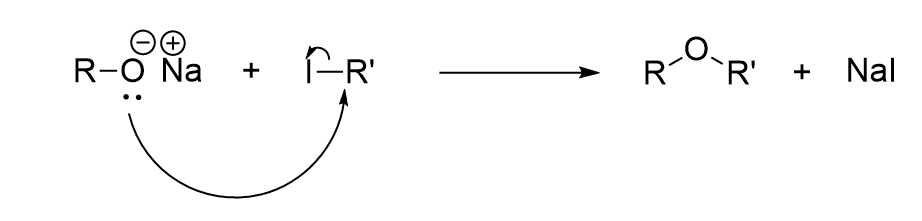
\includegraphics[width=0.8\linewidth]{Bilder/Williamsonsche-Ethersynthese.png}
\end{figure}
Diese Reaktion gilt analog für thiolate (Salz von Thiolen) um Thioether zu bilden. Diese Thioether können erneut alkyliert werden um Trialkylsulfoniumsalze zu bilden.

\subsubsection{Etherspaltung}
\begin{figure}[H]
	\centering
	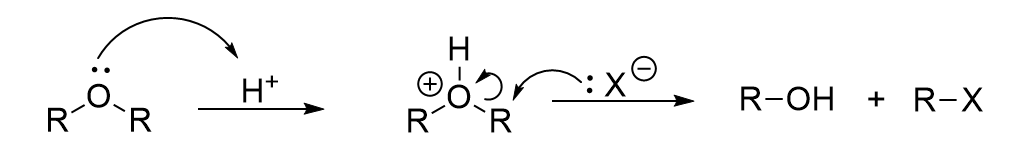
\includegraphics[width=0.8\linewidth]{Bilder/Saure-Etherspaltung.png}
\end{figure}

\subsubsection{Schmidt-Abbau}
\begin{figure}[H]
	\centering
	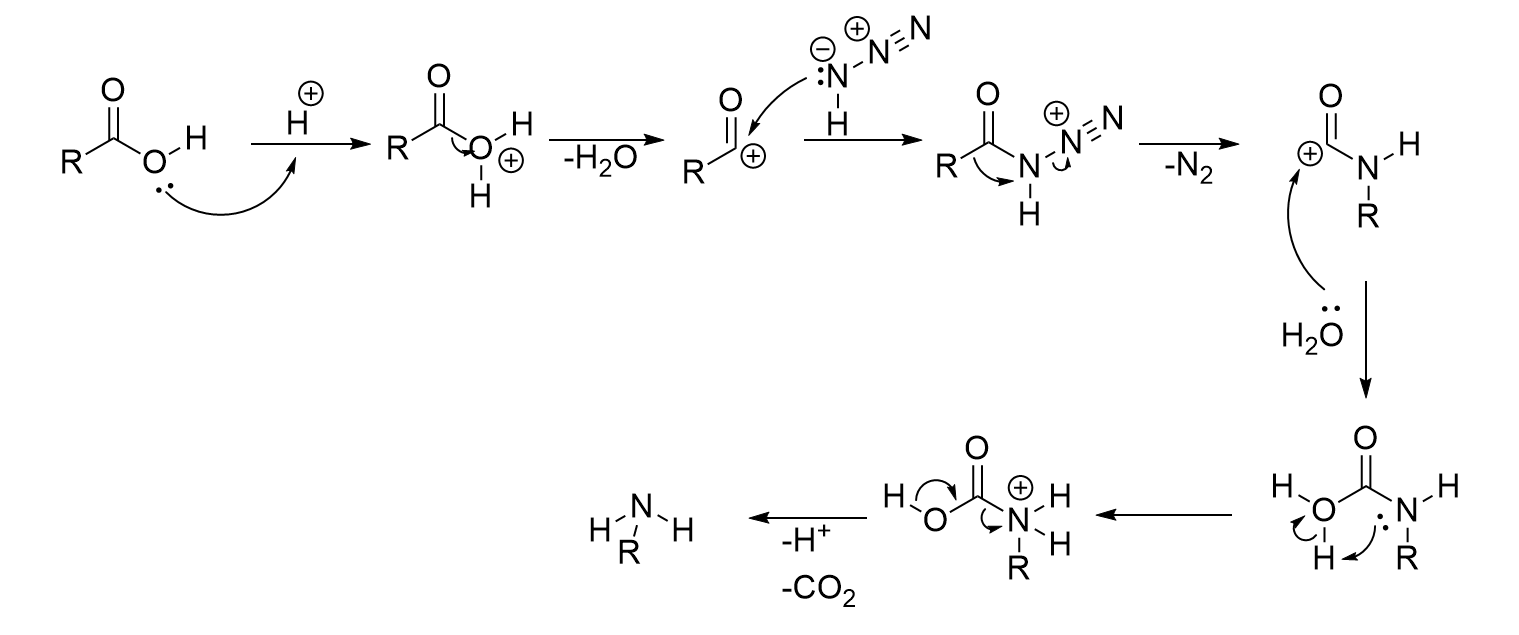
\includegraphics[width=\linewidth]{Bilder/Schmidt-Abbau.png}
\end{figure}

\subsubsection{Acylierung von Aminen}
\begin{figure}[H]
	\centering
	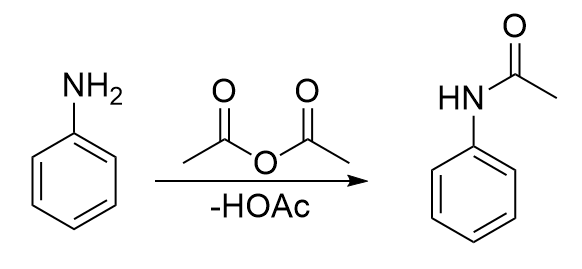
\includegraphics[width=0.4\linewidth]{Bilder/Acylierung von Aminen.png}
\end{figure}


\subsubsection{Hinsberg-Trennung von primären und sekundären Aminen}
\begin{figure}[H]
	\centering
	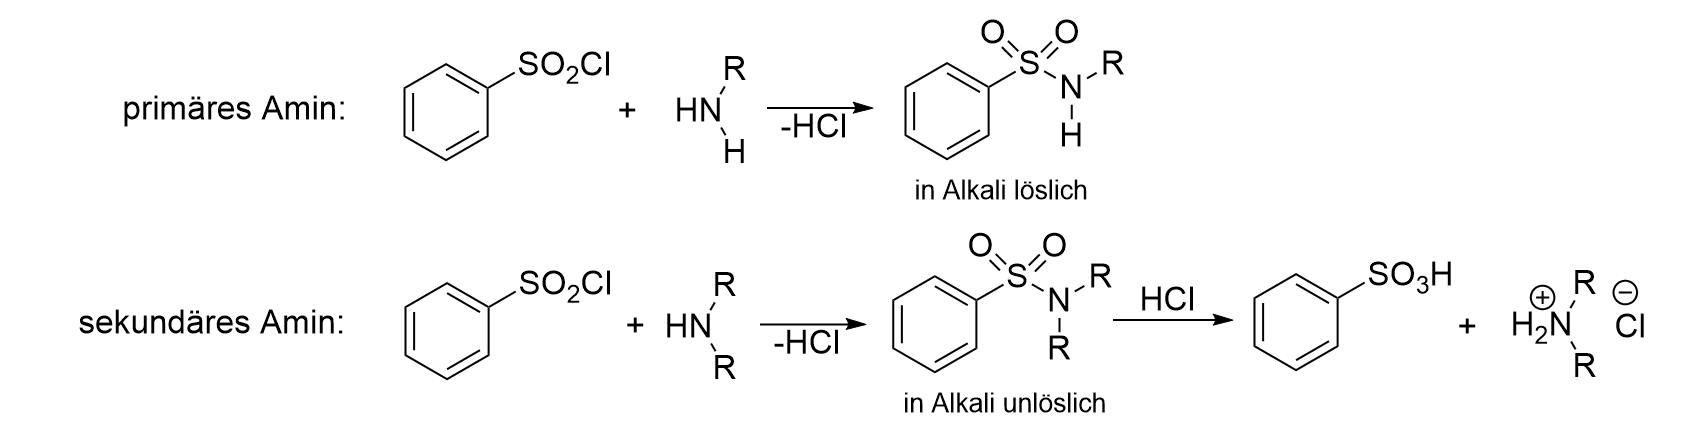
\includegraphics[width=1.1\linewidth]{Bilder/Hinsberg-Trennung.png}
\end{figure}


\subsection{Sonstiges}
%\subsubsection{Polymerisationsreaktionen}


\subsubsection{Simmons-Smith-Reaktion}
\begin{figure}[H]
    \centering
    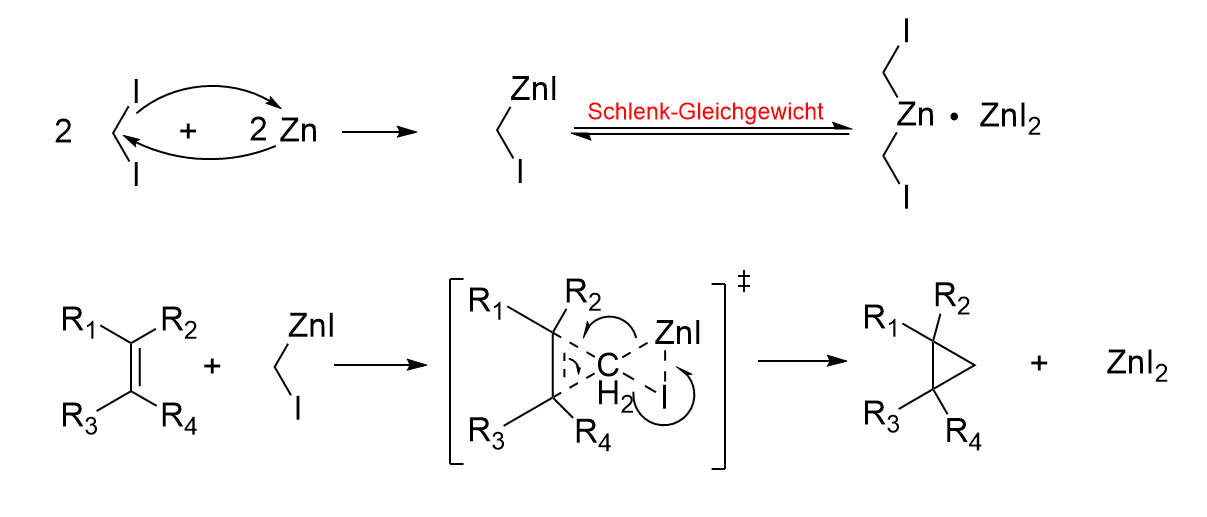
\includegraphics[width=\linewidth]{Bilder/simmons-smith.png}
\end{figure}


\subsubsection{Veresterung mit Diazomethan}
\subsubsection*{Darstellung von Diazomethan}
\begin{figure}[H]
	\centering
	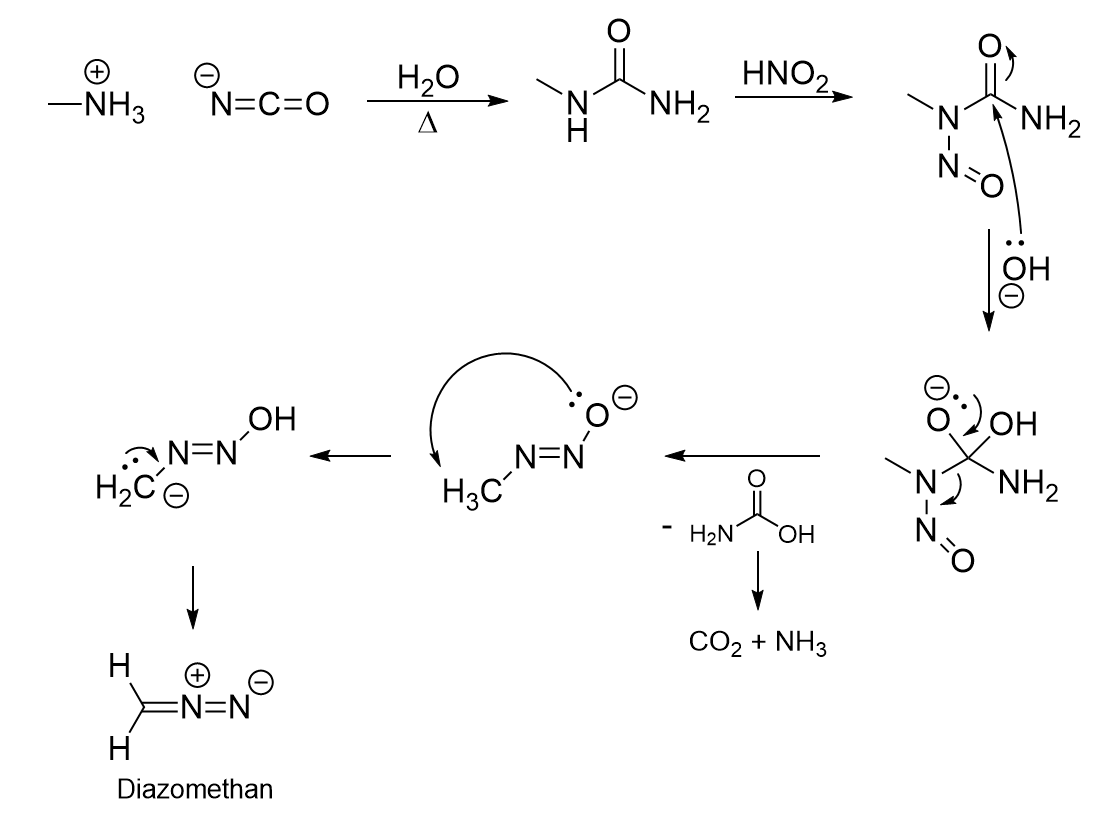
\includegraphics[width=0.8\linewidth]{Bilder/darstellung diazomethan.png}
\end{figure}
Diazomethan ist ein starkes Elektrophil und Alkylierungsmittel.
\subsubsection*{Umsetzung von Diazomethan mit Carbonsäuren}
\begin{figure}[H]
	\centering
	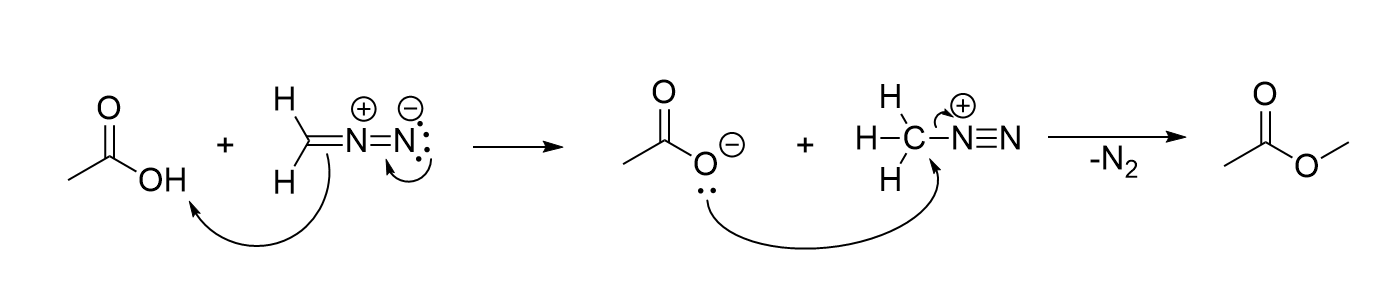
\includegraphics[width=0.9\linewidth]{Bilder/veresterung mit diazomethan.png}
\end{figure}

\subsection{Hofmann-Umlagerung}
\begin{figure}[H]
	\centering
	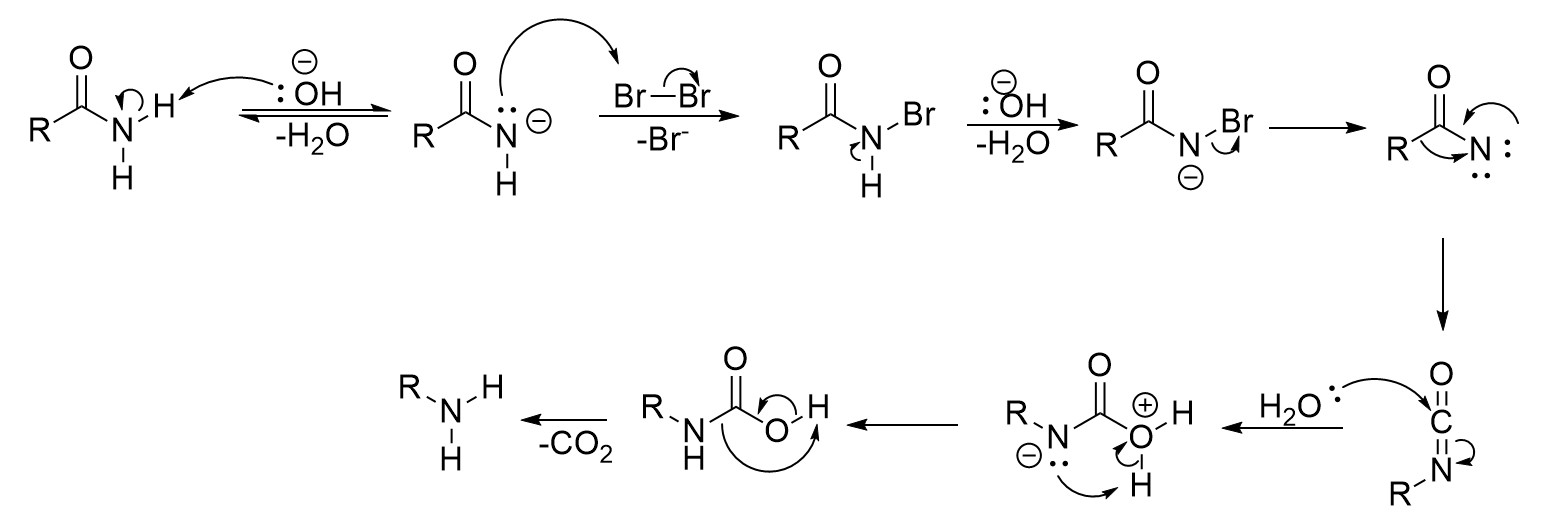
\includegraphics[width=\linewidth]{Bilder/Hofmann-Umlagerung.png}
\end{figure}

\subsubsection{Metallorganik}
\ce{M} steht in allen Nachfolgenden Reaktionen für ein Metall.
\subsubsection*{Wasserempfindlichkeit von Metallorganylen}
\begin{figure}[H]
	\centering
	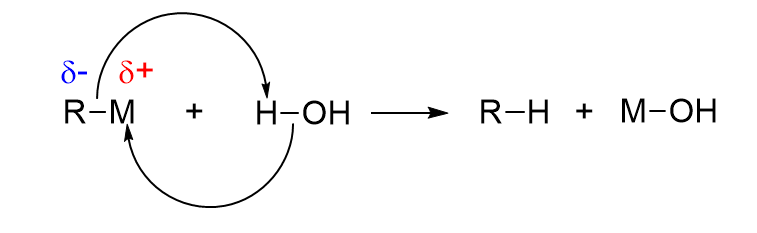
\includegraphics[width=0.6\linewidth]{Bilder/wasserempfindlichkeit Metallorganyle.png}
\end{figure}
\subsubsection*{Schlenk-Gleichgewicht}
\begin{figure}[H]
	\centering
	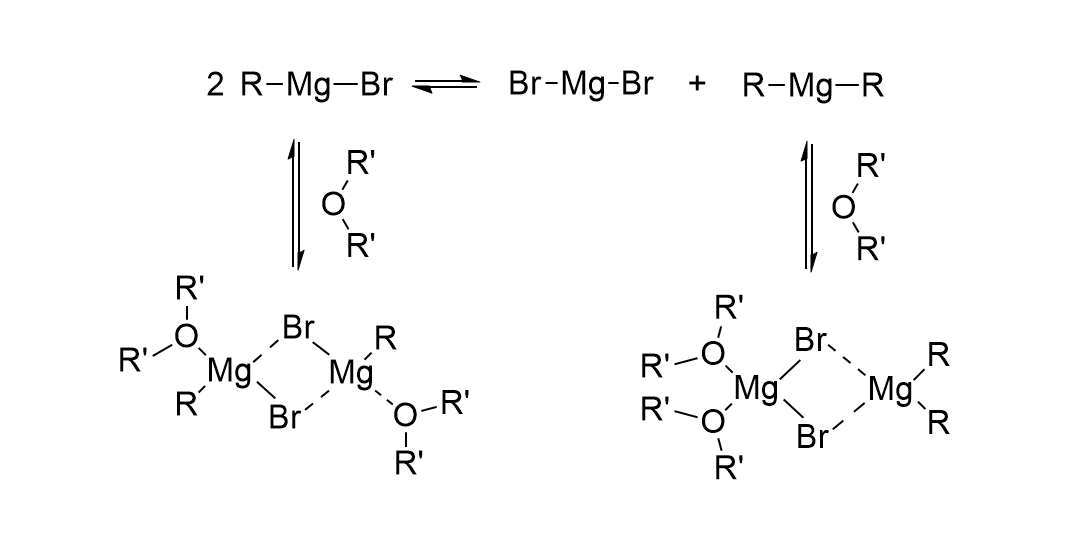
\includegraphics[width=0.9\linewidth]{Bilder/Schlenk Gleichgewicht.png}
\end{figure}


\subsubsection*{Synthese von Organolithiumverbindungen}
\begin{figure}[H]
	\centering
	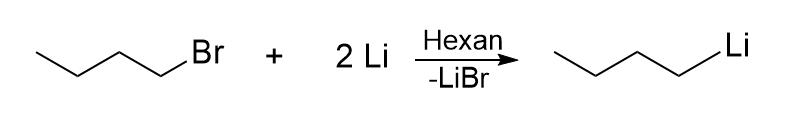
\includegraphics[width=0.7\linewidth]{Bilder/Synthese von Organolithiumverbindungen.png}
\end{figure}

\subsubsection*{Synthese von Grignard Verbindungen}
\begin{figure}[H]
	\centering
	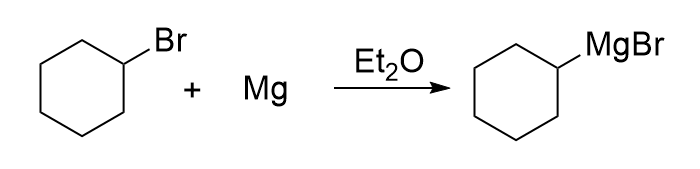
\includegraphics[width=0.6\linewidth]{Bilder/Synthese von Grignard-Verbindungen.png}
\end{figure}

\subsubsection*{Reaktion von Grignard Verbingungen mit Carbonylen}
\begin{figure}[H]
	\centering
	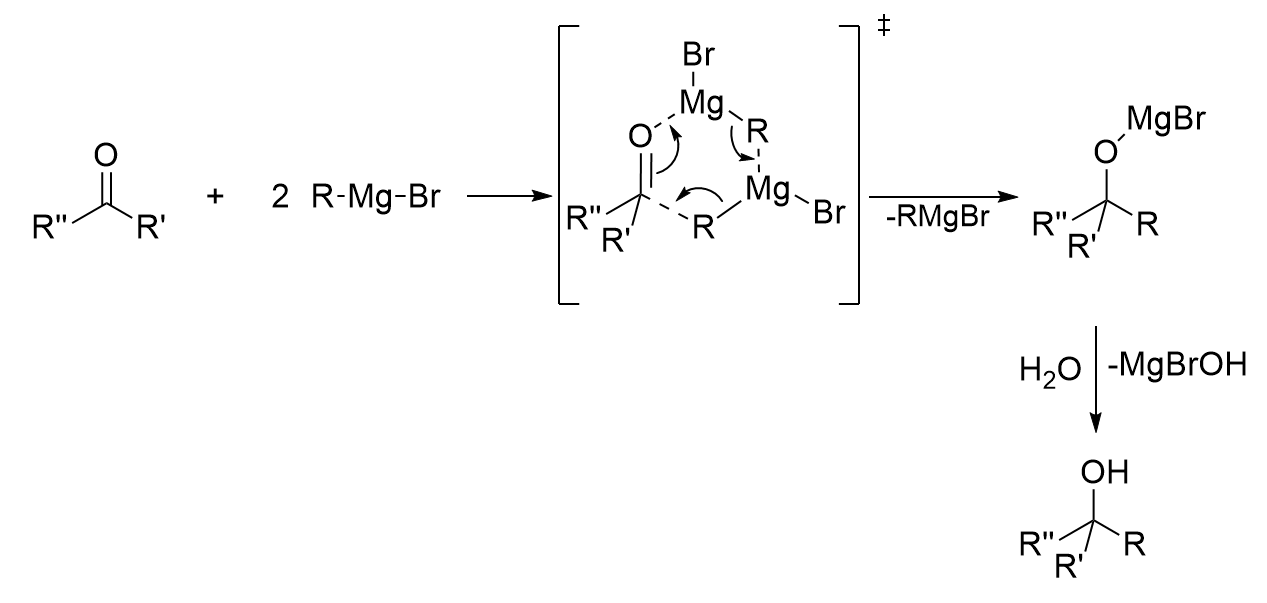
\includegraphics[width=\linewidth]{Bilder/Gringard mit Carbonylen.png}
\end{figure}
Aus Carbonylen entstehen Alkohole. Je nach Anzahl der Alkyl-Substituenten entstehen primäre, sekundäre oder tertiäre Alkohole.\\
 
 \noindent Werden Ester statt Aldehyde oder Ketone verwendet so existiert das Alkoholat als Abgangsgruppe. Somit wird der Carbonyl-Kohlenstoff zuerst einmal Alkyliert, wobei die Abgangsgruppe als Alkoholat abgespalten wird und sich die \chemfig{C=O} Carbonyl-Bindung wieder ausbildet. Dieses Carbonyl-Kohlenstoff wird nun erneut Alkyliert wobei der Alkohol entsteht, es wird also zweimal Alkyliert.



\subsubsection{Reduktionen}
\subsubsection*{Hydrierung von Mehrfachbindungen}
\begin{figure}[H]
	\centering
	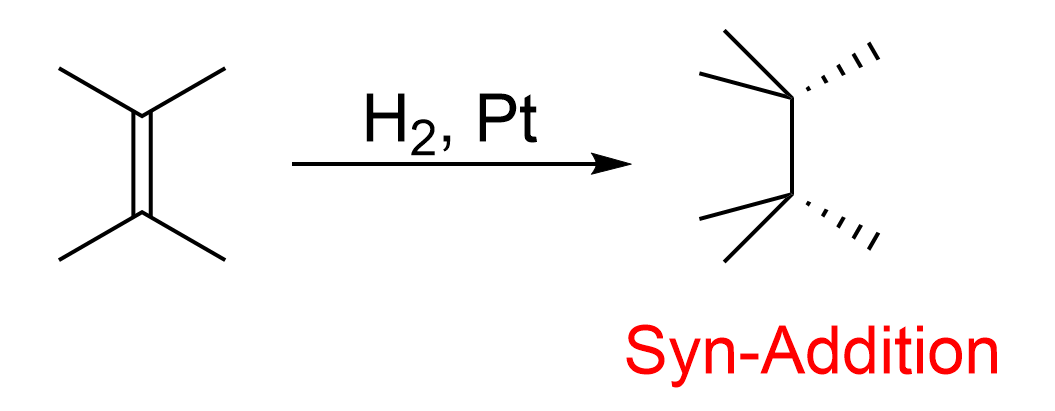
\includegraphics[width=0.5\linewidth]{Bilder/Hydrierungen von Mehrfachbindungen.png}
\end{figure}

\begin{figure}[H]
	\centering
	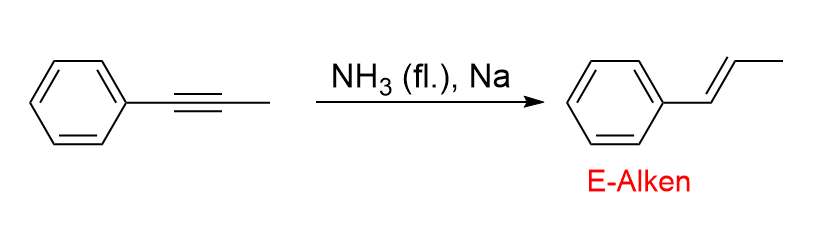
\includegraphics[width=0.7\linewidth]{Bilder/Hydrierung zum E-Alken.png}
\end{figure}
\begin{figure}[H]
	\centering
	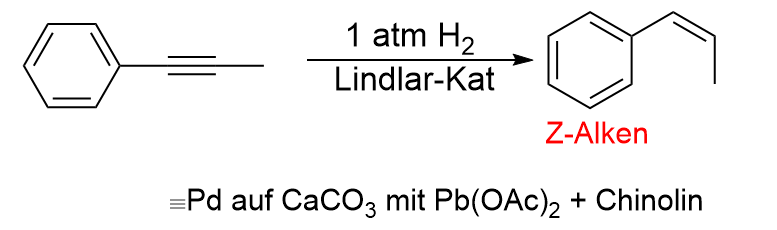
\includegraphics[width=0.7\linewidth]{Bilder/Hydrierung zum Z-Alken.png}
\end{figure}

\subsubsection*{Reduktion von Carbonylen}
\begin{figure}[H]
	\centering
	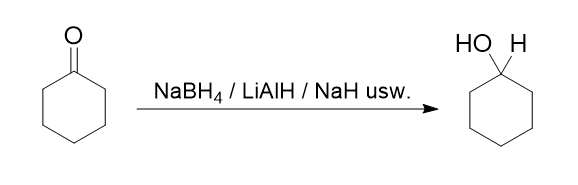
\includegraphics[width=0.7\linewidth]{Bilder/reduktion von carbonylen.png}
\end{figure}
\begin{figure}[H]
	\centering
	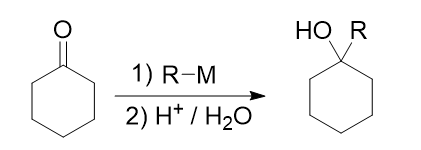
\includegraphics[width=0.5\linewidth]{Bilder/reduktion von carbonylen mit organometallen.png}
\end{figure}

\subsubsection*{Reduktion von Benzolsulfochlorid}
\begin{figure}[H]
	\centering
	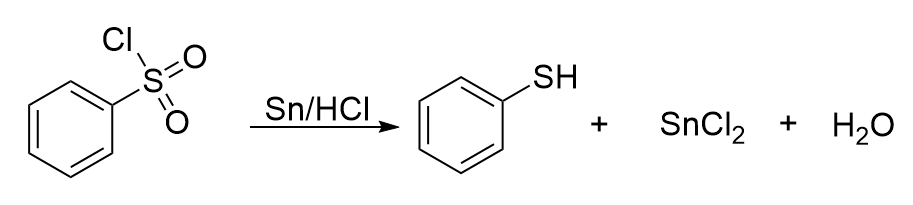
\includegraphics[width=0.8\linewidth]{Bilder/Reduktion von Benzosulfochlorid.png}
\end{figure}


\subsubsection*{Darstellung und Reduktion von Aziden}
\begin{figure}[H]
	\centering
	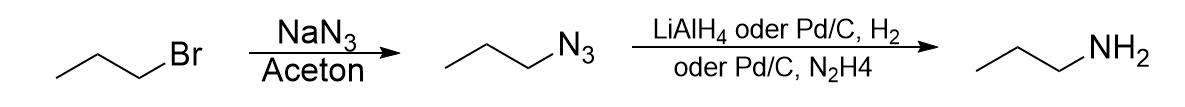
\includegraphics[width=\linewidth]{Bilder/Darstellung und Reduktion von Aziden.png}
\end{figure}

\subsubsection*{Reduktion von Amiden und Nitrilen}
\begin{figure}[H]
	\centering
	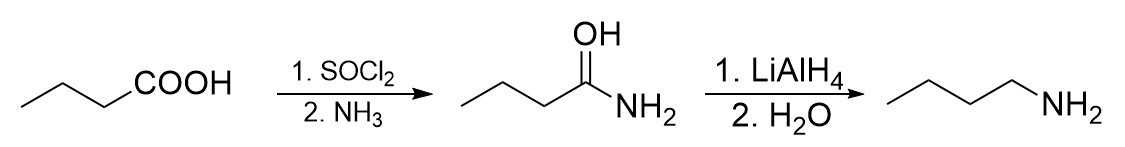
\includegraphics[width=0.9\linewidth]{Bilder/Reduktion von Amiden.png}
\end{figure}
\begin{figure}[H]
	\centering
	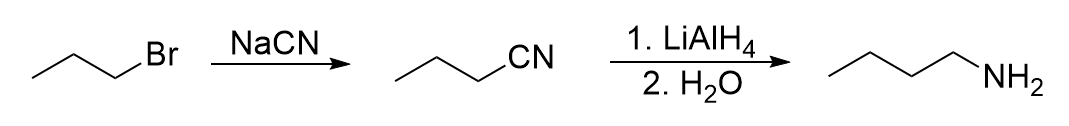
\includegraphics[width=0.9\linewidth]{Bilder/Reduktion von Nitrilen.png}
\end{figure}


\subsubsection*{Curtis-Abbau}
\begin{figure}[H]
	\centering
	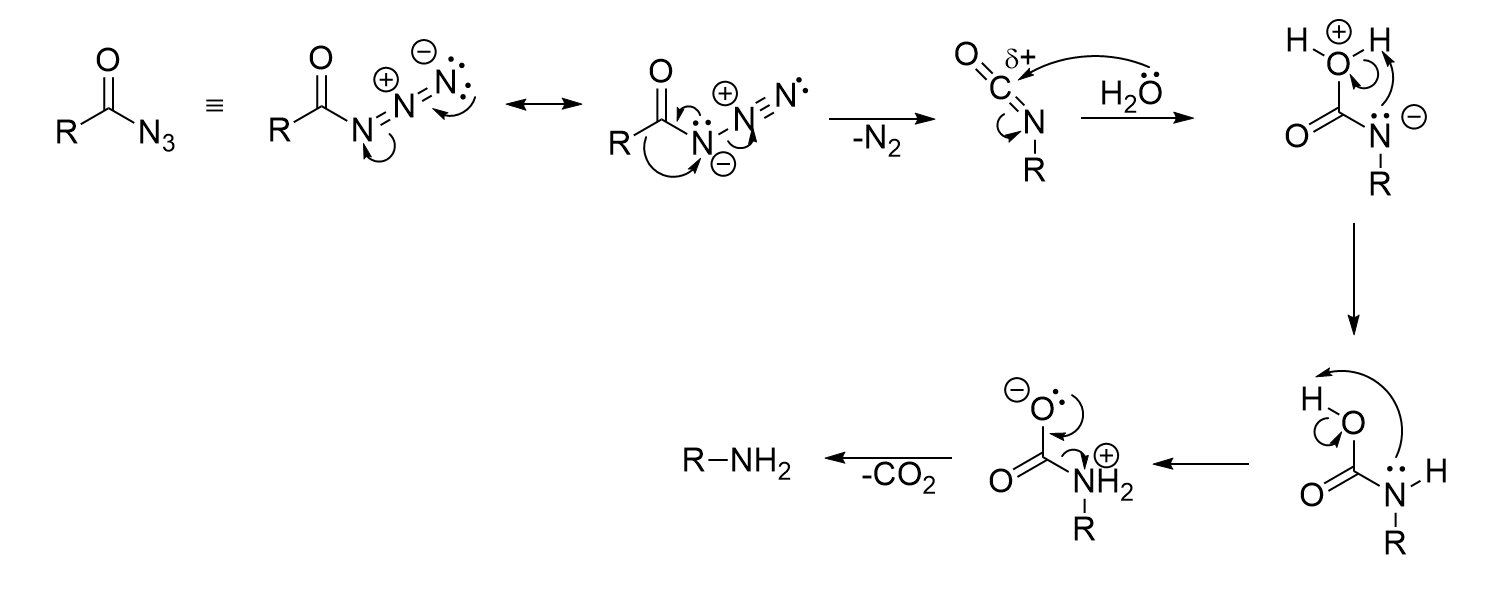
\includegraphics[width=\linewidth]{Bilder/curtis-abbau.png}
\end{figure}

\subsubsection*{Reduktive Aminierung}
\begin{figure}[H]
	\centering
	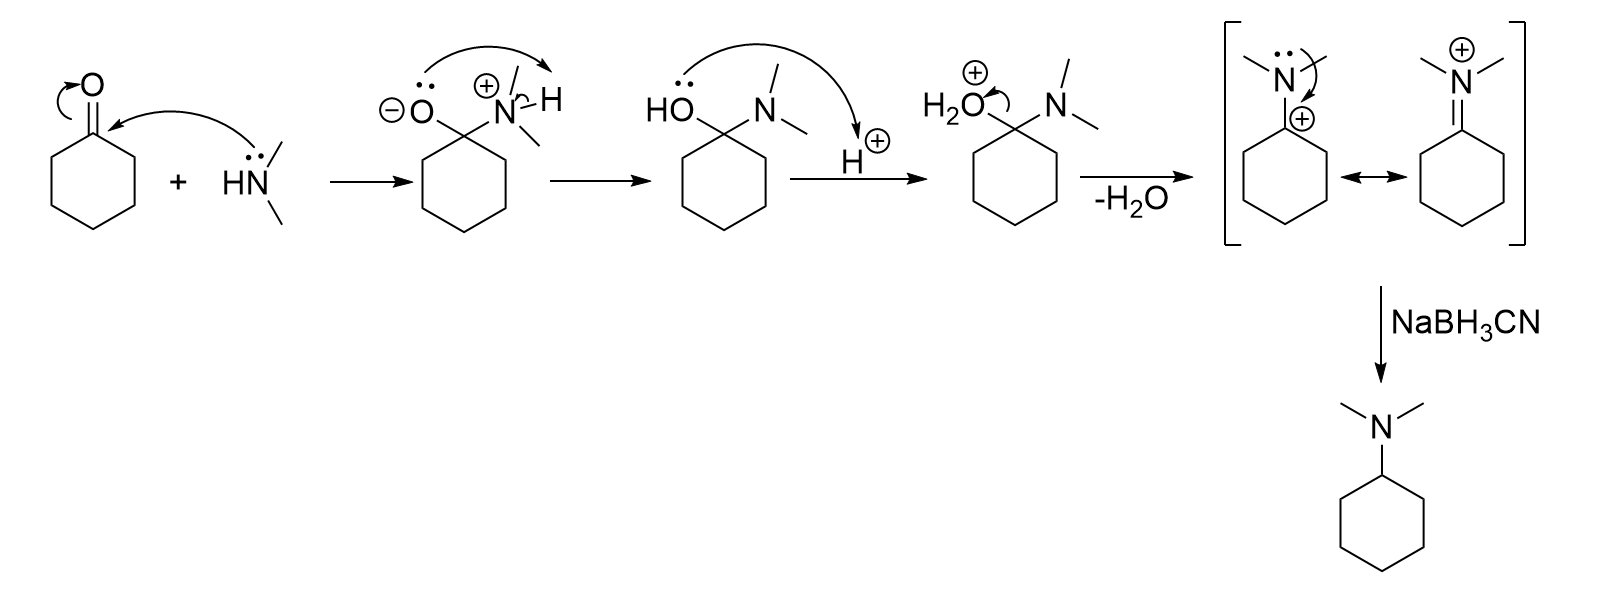
\includegraphics[width=\linewidth]{Bilder/reduktive aminierung 1.png}
\end{figure}
Beispiel Anwendung zur Reduktiven Aminierung:
\begin{figure}[H]
	\centering
	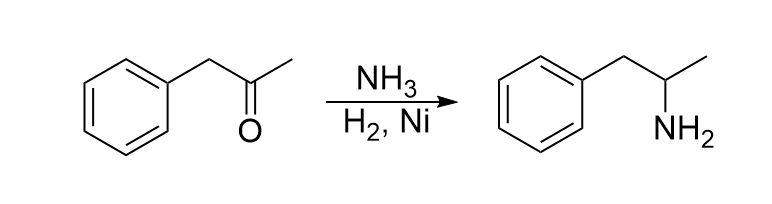
\includegraphics[width=0.6\linewidth]{Bilder/Reduktive Aminierung-Anwendung.png}
\end{figure}

\subsubsection{Oxidationen}
\subsubsection*{Oxidationen von Alkoholen}
\begin{figure}[H]
	\centering
	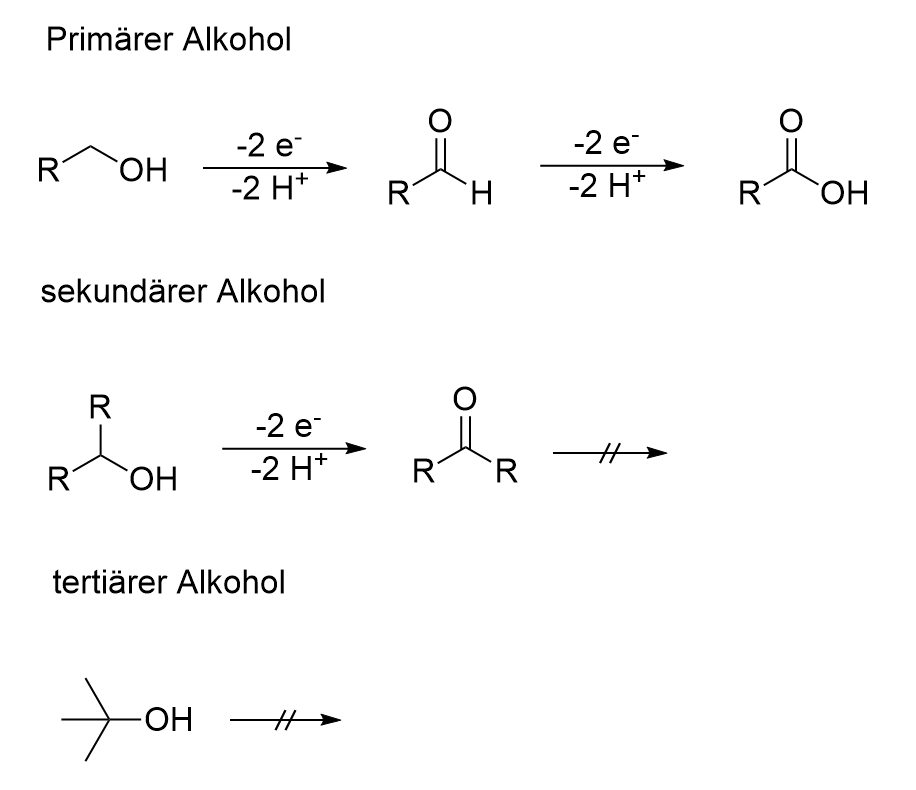
\includegraphics[width=0.8\linewidth]{Bilder/oxidation Alkohole.png}
\end{figure}

\subsubsection*{Milde Oxidation von Thiolen zu Disulfiden}
\begin{figure}[H]
	\centering
	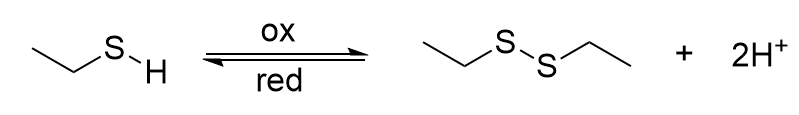
\includegraphics[width=0.8\linewidth]{Bilder/milde oxidation von Thiolen zu disulfiden.png}
\end{figure}

\subsubsection*{Starke Oxidation von Thiolen}
\begin{figure}[H]
	\centering
	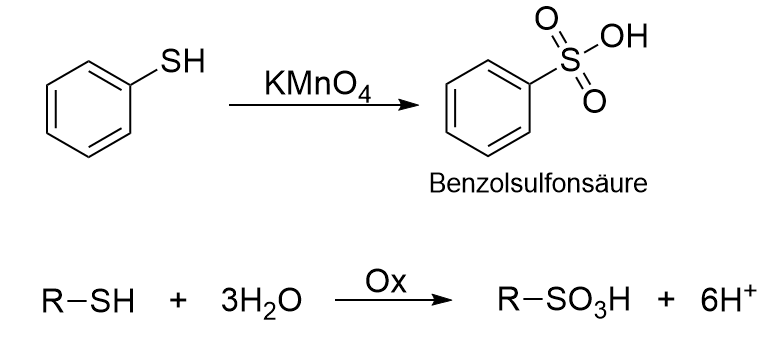
\includegraphics[width=0.7\linewidth]{Bilder/starke oxidation von thiolen.png}
\end{figure}


\subsubsection*{Oxidation von Thioethern}
\begin{figure}[H]
	\centering
	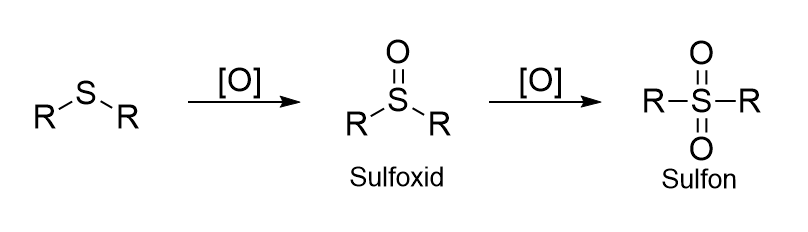
\includegraphics[width=0.7\linewidth]{Bilder/Oxidation von Thioethern.png}
\end{figure}
Die Erste Oxidation kann mit wässriger Wasserstoffperoxid-Lösung bei Raumtemperatur ablaufen. Für die zweite Oxidation zum Sulfon können als Reagenz Hydroperoxide (\ce{RCOOOH}) verwendet werden.

\subsubsection*{Oxidation von Aminen}
\begin{figure}[H]
	\centering
	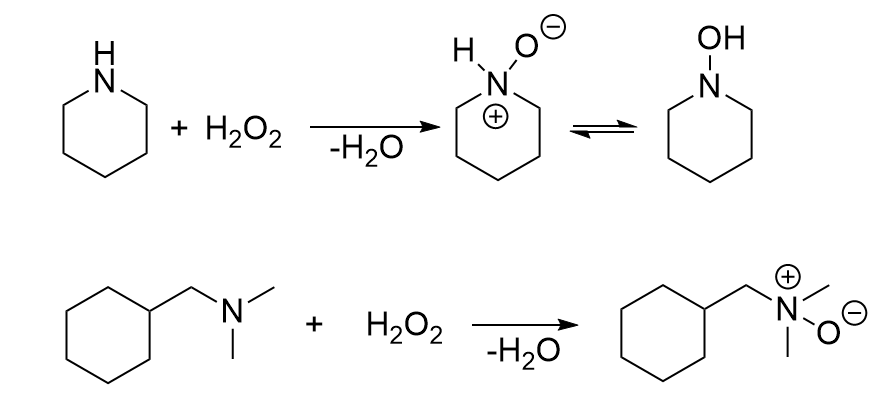
\includegraphics[width=0.7\linewidth]{Bilder/Oxidation von Aminen.png}
\end{figure}




%%%%%%%%%%%%%%%%%%%%%%%%%%%%%%%%%%%%%%%%%%%%%%%%%%%%%%%%%%%%%%%%%%%%%%%%%
\newpage
\section{Aromatisch}
\subsection{Elektrophile Substitution am Aromaten\label{sec:allgemein Ar-SE}}
In folgender Abbildung ist die allgemeine Elektrophile Addition am Aromaten dargestellt.
\begin{figure}[H]
	\centering
	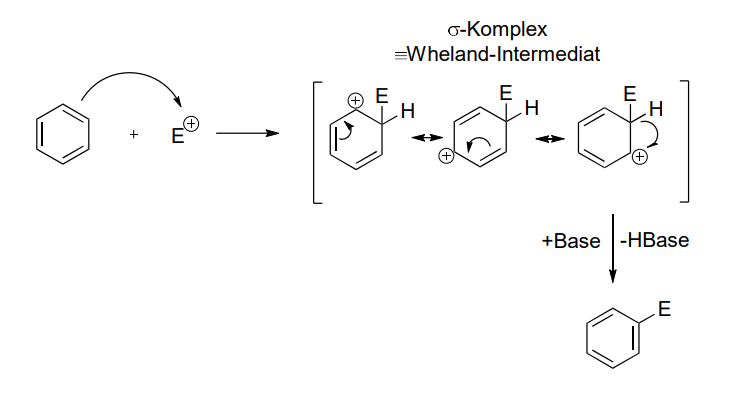
\includegraphics[width=\linewidth]{Bilder/Allgemeine Ar-SE.png}
\end{figure}
In den folgenden Unterüberschriften werden spezifische Elektrophile Aromatensubstitutionen aufgeführt.

\subsubsection{Nitrierung}
\begin{figure}[H]
	\centering
	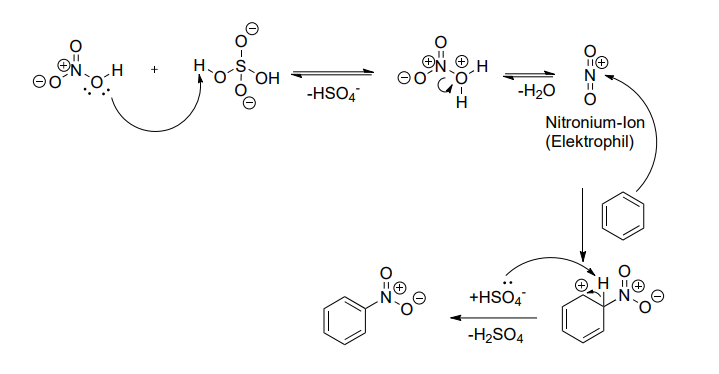
\includegraphics[width=\linewidth]{Bilder/Nitrierung.png}
\end{figure}

\subsubsection{Sulfonierung}
\begin{figure}[H]
	\centering
	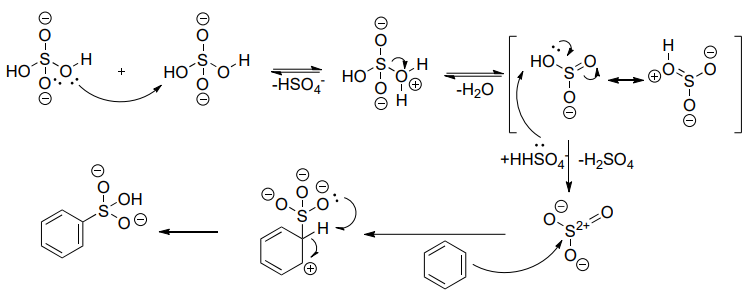
\includegraphics[width=\linewidth]{Bilder/Sulfonierung.png}
\end{figure}
\newpage
\subsubsection{Friedel-Crafts-Alkylierung}
Für den Mechanismus der Friedel-Crafts-Alkylierung mit primären oder sekundären Halogenalkanen gilt folgender Mechanismus. Für tertiäre Halogenalkane bildet sich das Elektrophil nach \ce{S_{N1}}.
\begin{figure}[H]
	\centering
	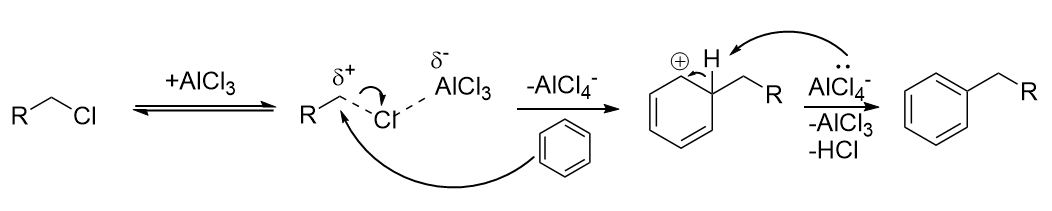
\includegraphics[width=\linewidth]{Bilder/Friedel-Crafts-Alkylierung_Metallhalogenid-Mechanismus.png}
\end{figure}
\noindent Das dadurch dargestellte Elektrophil kann analog zu \autoref{sec:allgemein Ar-SE} mit Aromaten reagieren.\\

\noindent Im Nachfolgenden sind weitere, sowie die schon für Metallhalogenid-Katalysatoren beschriebene Darstellungen von Friedel-Crafts-Elektrophilen aufgeführt.
\begin{figure}[H]
	\centering
	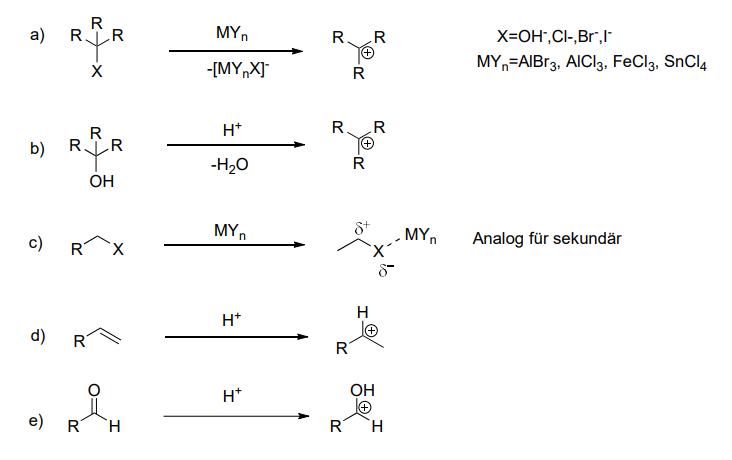
\includegraphics[width=\linewidth]{Bilder/Friedel-Crafts-Alkylierung.png}
\end{figure}

\subsubsection{Friedel-Crafts-Acylierung}
\begin{figure}[H]
	\centering
	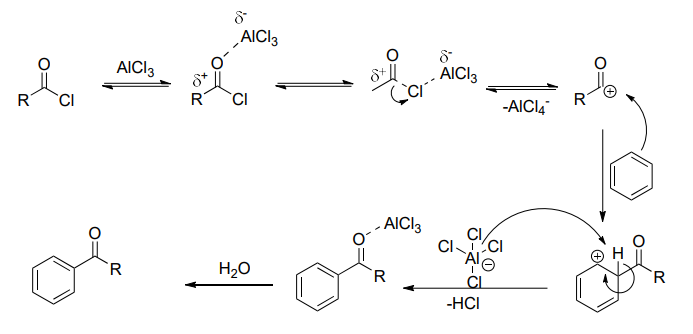
\includegraphics[width=\linewidth]{Bilder/Friedel-Crafts-Acylierung.png}
\end{figure}
Die Friedel-Crafts-Acylierung kann keine Aldehyde darstellen, da das hierfür erforderliche Reagenz instabil ist.

\subsubsection{Vilsmeyer-Hack-Formylierung}
Die Vilsmeyer-Hack-Formylierung ist eine Reaktion zur Darstellung von Aldehyden. Es werden bevorzugt \textit{para}-Produkte gebildet. Sie beschränkt sich auf elektronenreiche Aromaten wie Phenole, Amine oder Furane.
\subsubsection*{Reaktionsgleichung}
Gezeigt ist die Reaktionsgleichung am Beispiel von \textit{N,N-Dimethylanilin}.
\begin{figure}[H]
	\centering
	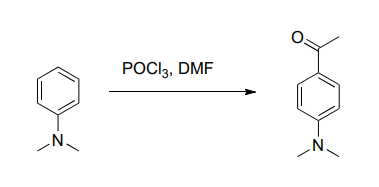
\includegraphics[width=0.6\linewidth]{Bilder/Vilsmeyer-Hack-Formylierung-Reaktionsgleichung.png}
\end{figure}
\subsubsection*{Mechanismus}
Gezeigt ist der Mechanismus am Beispiel von \textit{N,N-Dimethylanilin}.
\begin{figure}[H]
	\centering
	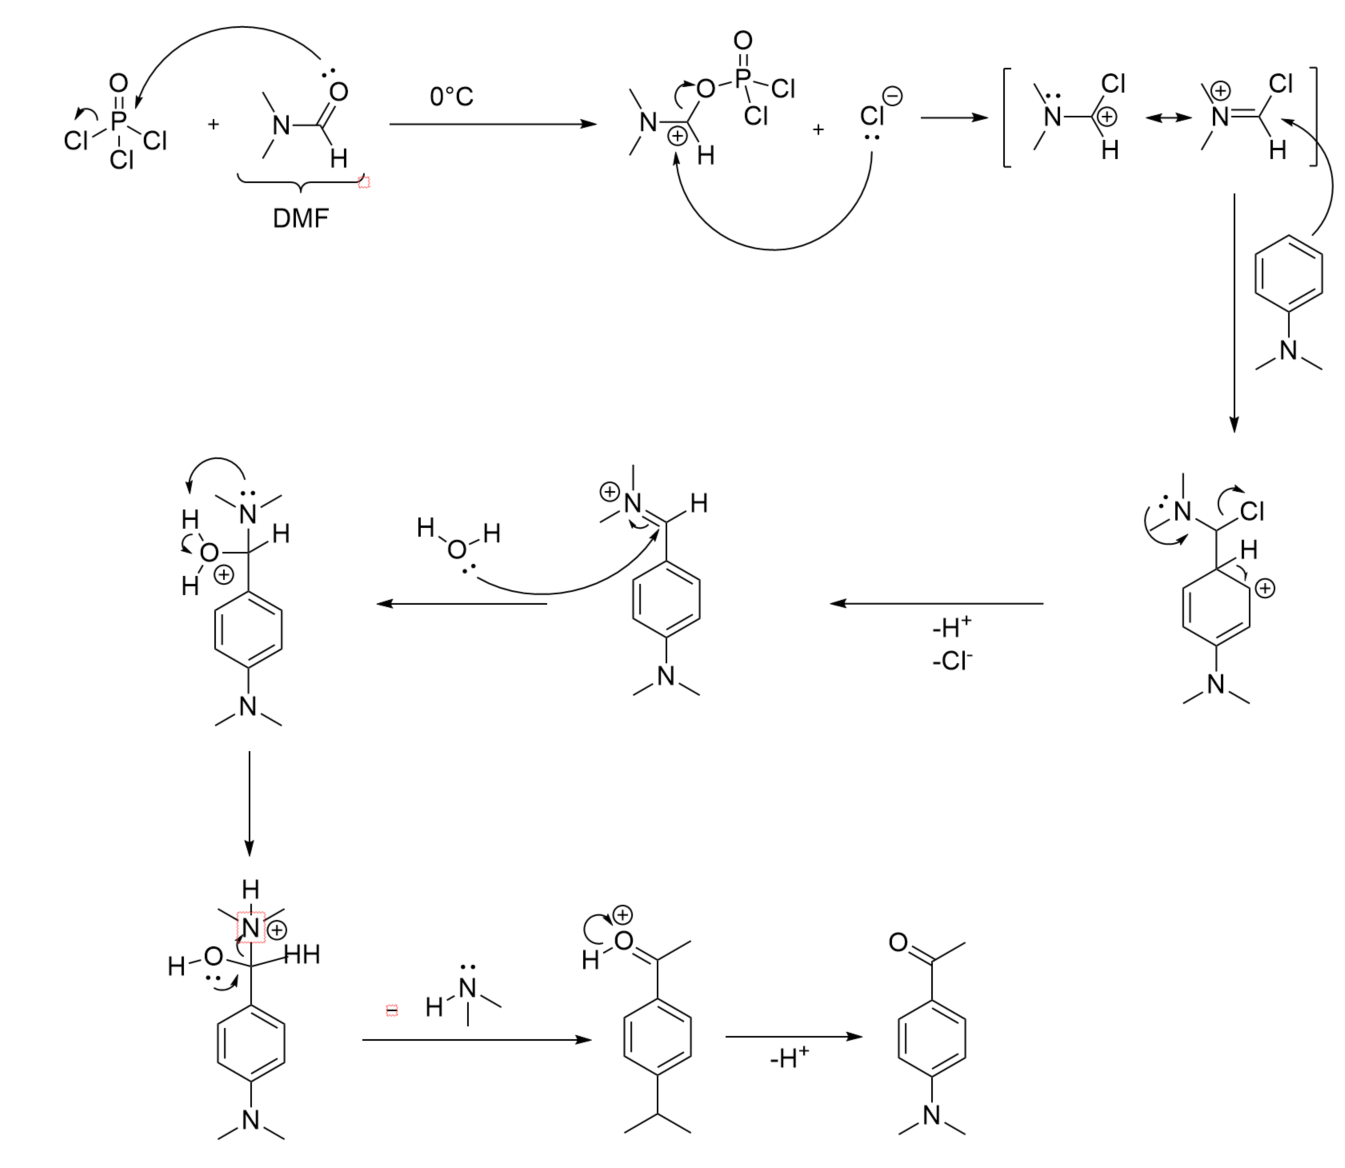
\includegraphics[width=\linewidth]{Bilder/Vilsmeier-Hack-Formylierung-Mechanismus.png}
\end{figure}

\newpage
\subsubsection{Kolbe-Schmitt}
\subsubsection*{Reaktionsgleichung}
Nachfolgend ist eine vereinfachte Reaktionsgleichung der Salicylsäure-Synthese dargestellt.
\begin{figure}[H]
	\centering
	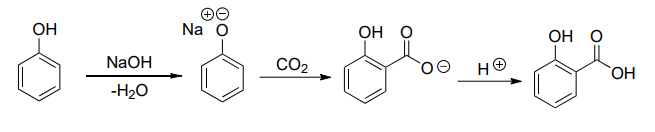
\includegraphics[width=0.9\linewidth]{Bilder/Kolbe-Schmitt-Salicylsäure.png}
\end{figure}

\subsubsection*{Mechanismus}
\begin{figure}[H]
	\centering
	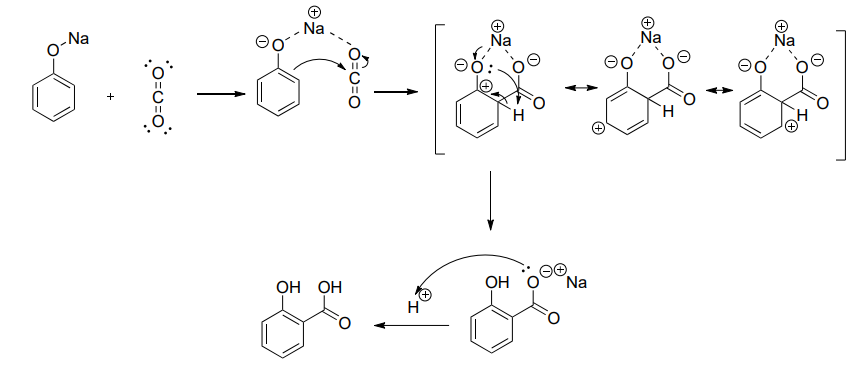
\includegraphics[width=\linewidth]{Bilder/Kolbe-Schmitt-Mechanismus.png}
\end{figure}

\subsubsection{Hooksche Phenolsynthese}
Die Hooksche Phenolsynthese dient zur Darstellung von Phenol und von Aceton als Nebenprodukt.
\begin{figure}[H]
	\centering
	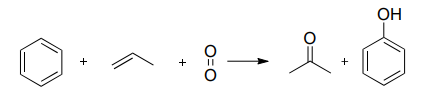
\includegraphics[width=0.7\linewidth]{Bilder/Hooksche-Phenolsynthese-Bilanzgleichung.png}
\end{figure}
\noindent Die Reaktion ist kein eigener Mechanismus, sondern eine Folge von bekannten Mechanismen.
\begin{enumerate}
    \item Friedel-Crafts-Alkylierung von Benzol mit Propen zu Cumol
    \item Das Cumol durchläuft eine Radikalische Substitution mit Radikalstartern und Sauerstoff als Reagenz. Dabei entsteht Cumolhydroperoxid
    \item Das Cumolhydroperoxid durchläuft eine Umlagerung, aus der sich Aceton und Phenol bilden.
\end{enumerate}
Der Mechanismus der Umlagerung ist nachfolgend aufgeführt.
\begin{figure}[H]
	\centering
	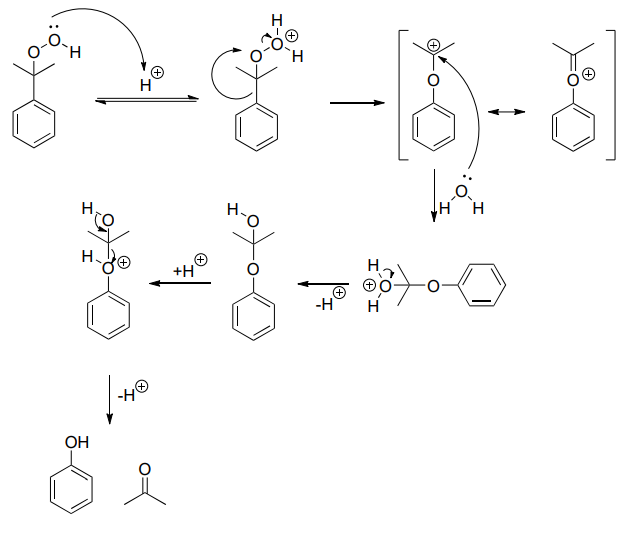
\includegraphics[width=0.9\linewidth]{Bilder/Hooksche-Phenolsynthese-Umlagerung.png}
\end{figure}

\subsection{Diazotierung und Azokupplung}
\subsubsection{Diazotierung}
\begin{figure}[H]
	\centering
	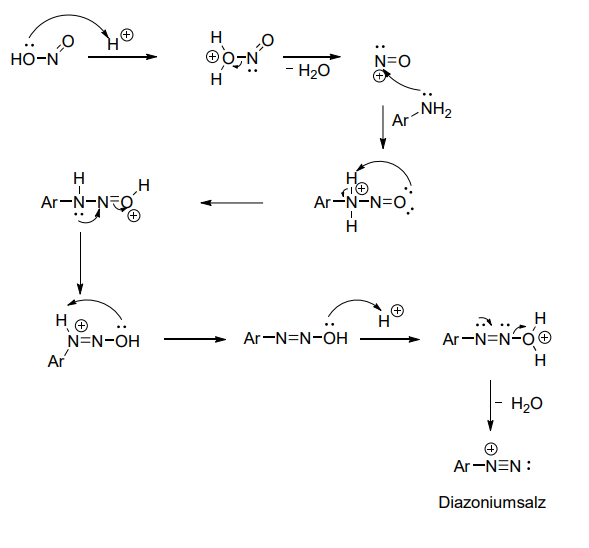
\includegraphics[width=0.8\linewidth]{Bilder/Diazotierung.png}
\end{figure}

\subsubsection{Azokupplung}
Der Mechanismus der Azokupplung folgt der allgemeinen elektrophilen Substitution am Aromaten. Das Elektrophil ist das durch Diazotierung dargestellte Diazonium-kation.\\

\noindent Für die Position des Angriffs sind die dirigierenden Substituenten verantwortlich.



\subsection{Reaktionen mit Diazoniumsalzen}
\subsubsection{Phenolverkochung}
\begin{figure}[H]
	\centering
	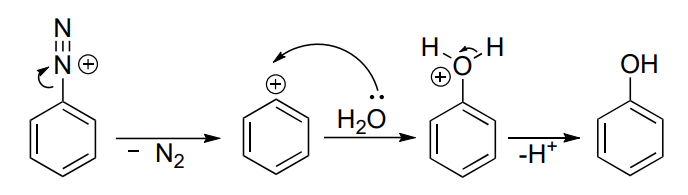
\includegraphics[width=0.7\linewidth]{Bilder/Phenolverkochung.png}
\end{figure}


\subsubsection{Sandmeyer-Reaktion}
\begin{figure}[H]
	\centering
	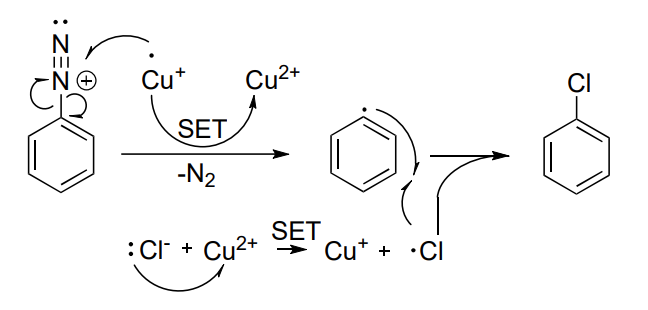
\includegraphics[width=0.7\linewidth]{Bilder/Sandmeyer-Mechanismus.png}
\end{figure}


\subsubsection{Schiemann-Reaktion}
\begin{figure}[H]
	\centering
	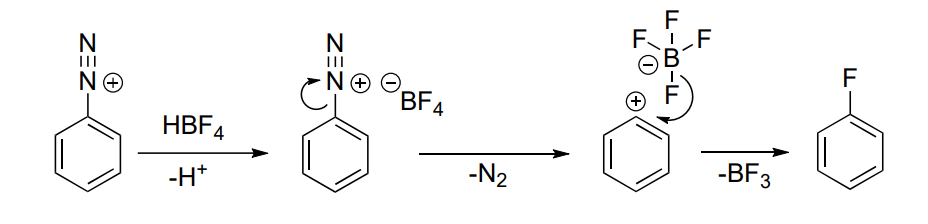
\includegraphics[width=\linewidth]{Bilder/Schiemann-Reaktion.png}
\end{figure}




\newpage
\subsection{Nucleophile Aromatische Substitution}
\subsubsection{Allgemein}
Für die Ar-\ce{S_N} ist es zwingend notwendig, dass der Aromat Elektronenarm ist, da Elektronenziehende Gruppen in \textit{ortho} und \textit{para} Positionen den Meisenheimer-Komplex stabilisieren.
\begin{figure}[H]
	\centering
	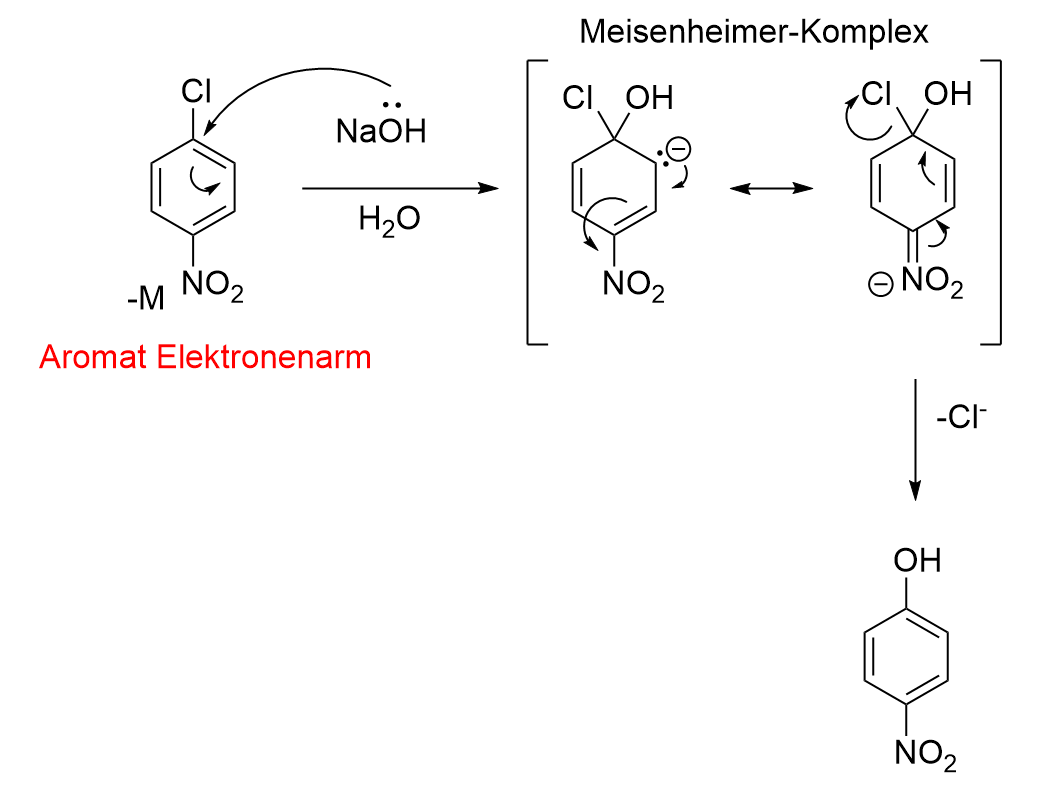
\includegraphics[width=0.85\linewidth]{Bilder/nucleophile-aromatische-Substitution.png}
\end{figure}

\subsubsection{Besondere Ar-\ce{S_N}}
\subsubsection*{Dow-Phenolprozess}
\begin{figure}[H]
	\centering
	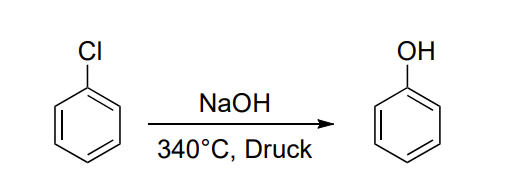
\includegraphics[width=0.53\linewidth]{Bilder/Dow-Phenolprozess.png}
\end{figure}

\subsubsection*{Darstellung von Aminen}
\begin{figure}[H]
	\centering
	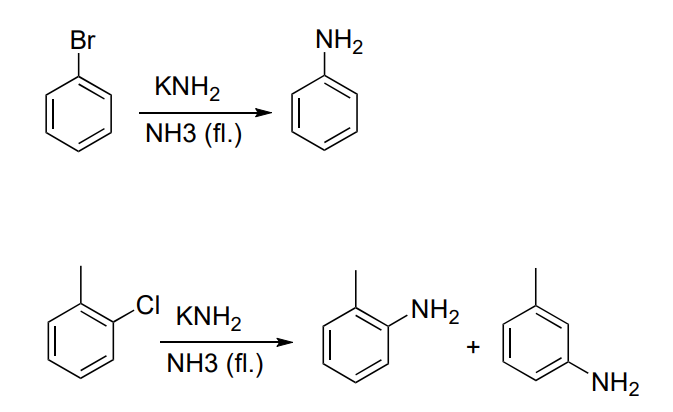
\includegraphics[width=0.7\linewidth]{Bilder/Ar-SE-Darstellung von Aminen.png}
\end{figure}
Die letzte Reaktion liefert zwei Konstitutionsisomere. Dies wird durch den Mechanismus der nachfolgend gezeigt ist klar.
\begin{figure}[H]
	\centering
	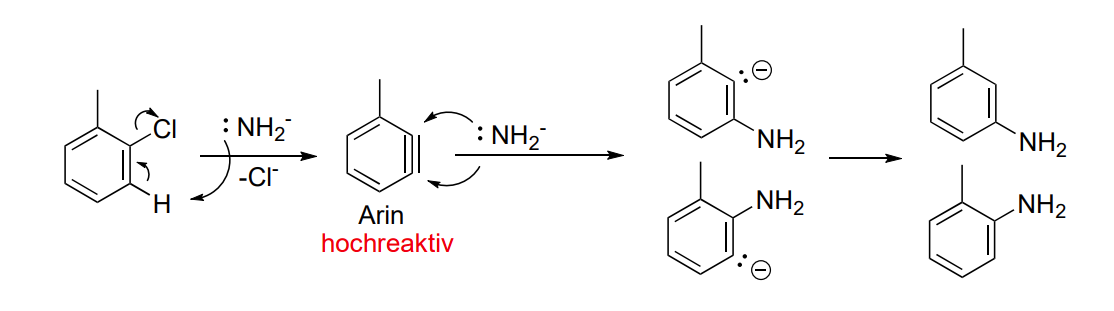
\includegraphics[width=\linewidth]{Bilder/Ar-SE-Darstellung von Aminen-Mechanismus.png}
\end{figure}

\subsection{Hydrierung von Aromaten}
\subsubsection{Vollständige Hydrierung mit Metallkatalysatoren}
\begin{figure}[H]
	\centering
	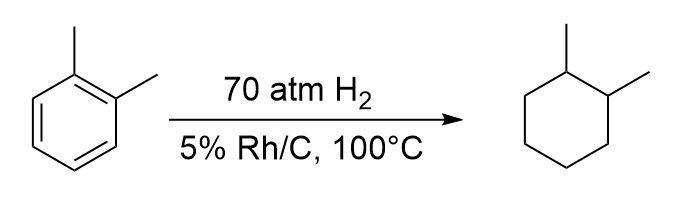
\includegraphics[width=0.65\linewidth]{Bilder/Hydrierung von Aromaten-1.png}
\end{figure}



\subsubsection{Birch-Reduktion von Aromaten}
\subsubsection*{Reaktionen}
\begin{figure}[H]
	\centering
	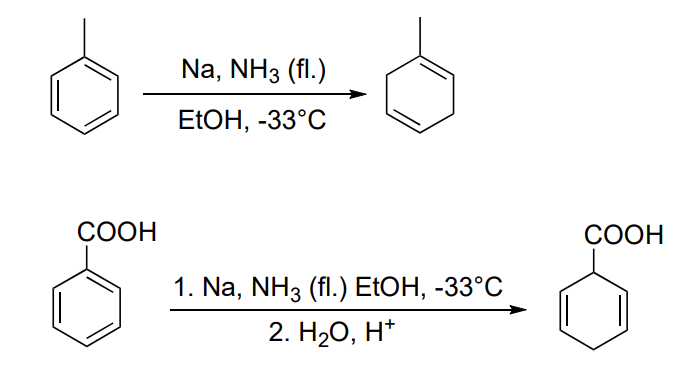
\includegraphics[width=0.75\linewidth]{Bilder/Birch-Reduktion-Reaktionen.png}
\end{figure}

\subsubsection*{Mechanismus}
\begin{figure}[H]
	\centering
	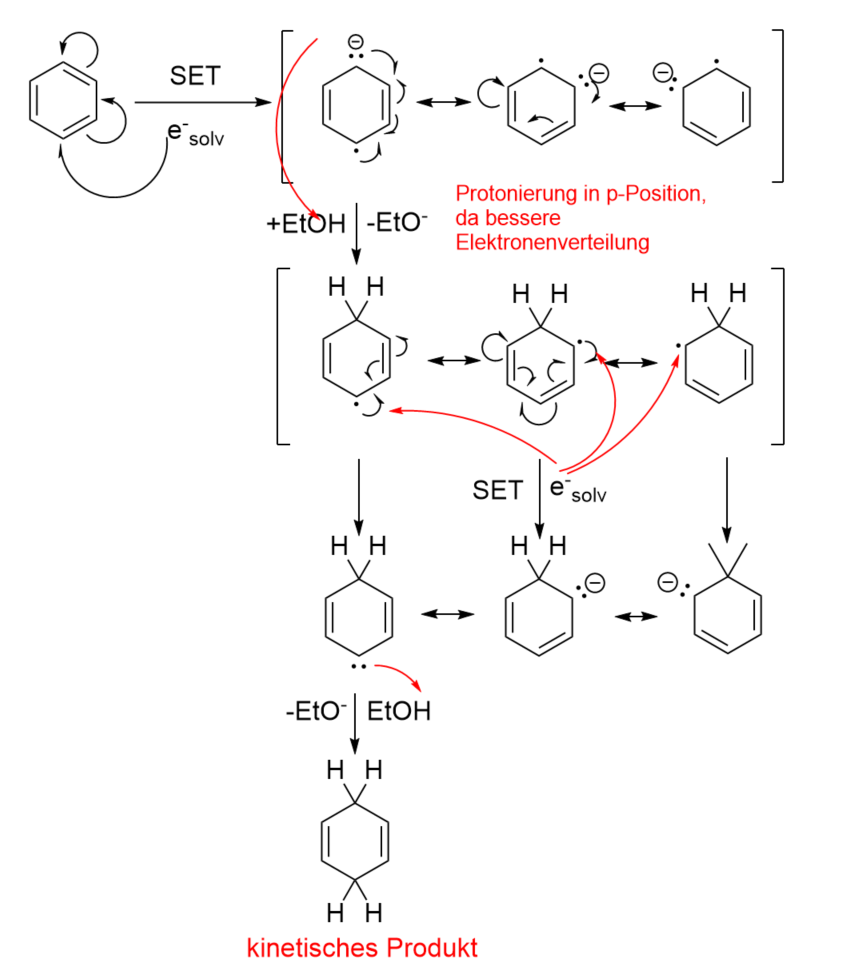
\includegraphics[width=0.9\linewidth]{Bilder/Birch-reduktion-mechanismus.png}
\end{figure}


\subsubsection{Reduktion der Nitro-Gruppe}
\subsubsection*{Katalytisch}
\begin{figure}[H]
	\centering
	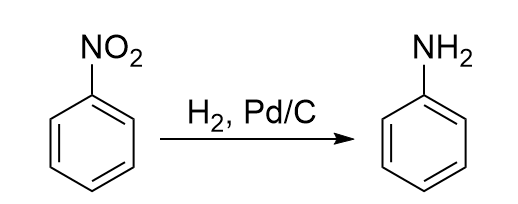
\includegraphics[width=0.5\linewidth]{Bilder/Reduktion der Nitro-Gruppe-Katalytisch.png}
\end{figure}
Die Nitro Gruppe kann zudem noch mit \ce{SnCl2} und konz. Salzsäure reduziert werden. Außerdem können Nitro-Gruppen mit Nickel und Wasserstoff (und Druck, Hitze) reduziert werden.

\subsubsection*{Clemmensen-artige Reduktion}
\begin{figure}[H]
	\centering
	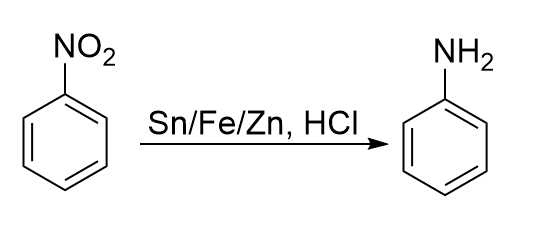
\includegraphics[width=0.5\linewidth]{Bilder/Clemmensen-artige-Reduktion.png}
\end{figure}

\subsection{Oxidation am Aromaten}
\subsubsection{Oxidation von Alkyl-Substituenten}
\begin{figure}[H]
	\centering
	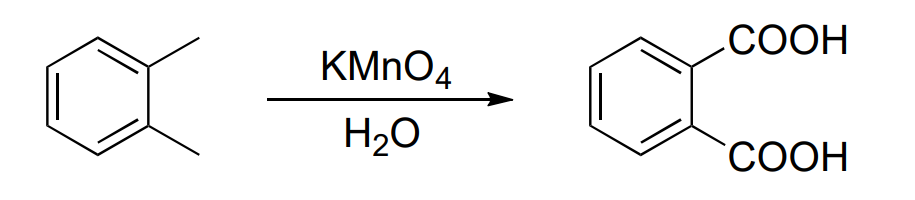
\includegraphics[width=0.6\linewidth]{Bilder/oxidation von xylol.png}
\end{figure}
\noindent Handelt es sich bei den Alkylsubstituenten nicht um Methyl-Substituenten, so entsteht trotzdem ein Benzoesäure derivat, da die Oxidation über Benzyl-Radikale verläuft und diese am stabilsten sind. Somit wird jegliche Kohlenstoffkette überhalb der benzylischen Position gespalten.
\begin{figure}[H]
	\centering
	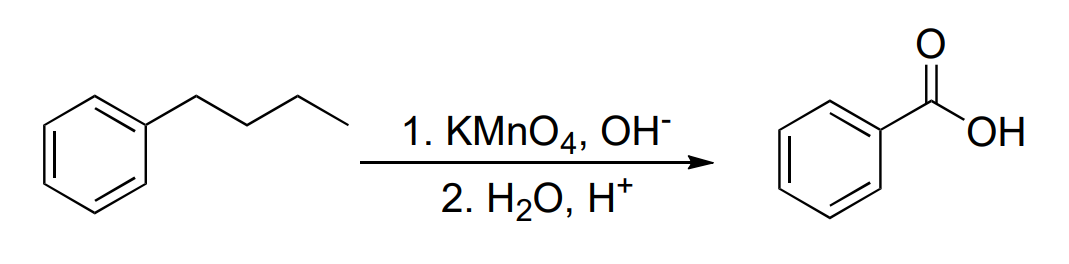
\includegraphics[width=0.7\linewidth]{Bilder/benzylische Oxidation.png}
\end{figure}
\subsubsection{Selektive benzylische Oxidation}
\begin{figure}[H]
	\centering
	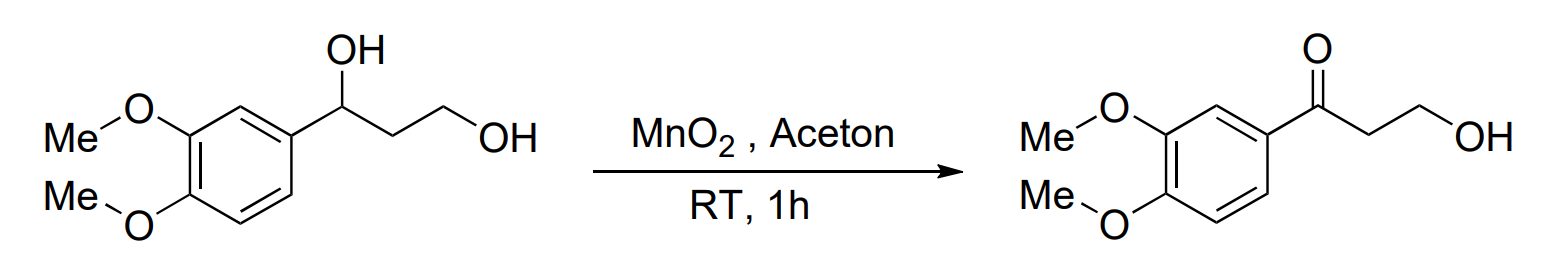
\includegraphics[width=\linewidth]{Bilder/selektive benzylische Oxidation.png}
\end{figure}




\subsection{Besonderheiten von Phenolen}
\subsubsection{Oxidaton von Phenolen zu Chinonen}
\begin{figure}[H]
	\centering
	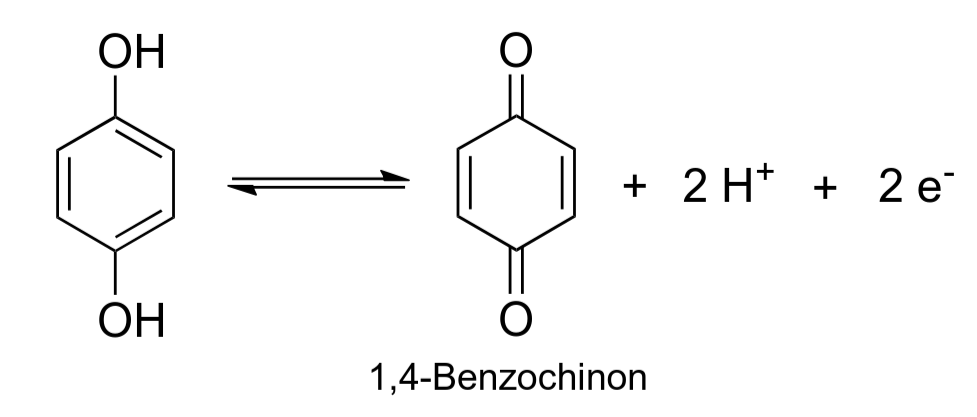
\includegraphics[width=0.5\linewidth]{Bilder/Phenol-Chinon-GGW.png}
\end{figure}
\subsubsection{Spezialfall der Bromierung von Phenolen}
\begin{figure}[H]
	\centering
	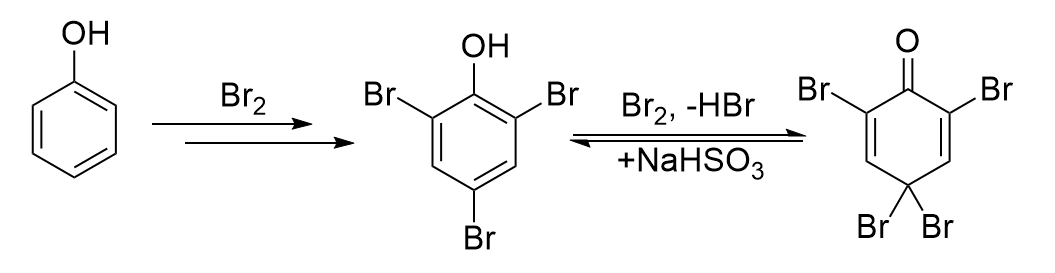
\includegraphics[width=0.75\linewidth]{Bilder/Bromierung von Phenol.png}
\end{figure}

\subsubsection{Reimer Tiemann-Reaktion}
Darstellung des Reagenz: \ce{HCCl3 + ^-OH -> ^-CCl3 + H2O -> CCl2 + Cl^-}
\begin{figure}[H]
	\centering
	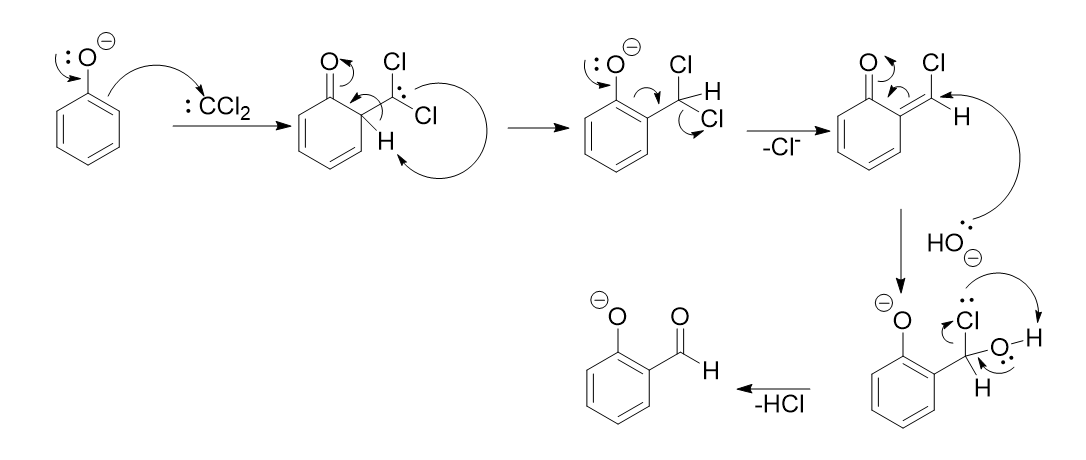
\includegraphics[width=\linewidth]{Bilder/Reimer-Tiemann-Reaktion.png}
\end{figure}

\subsubsection{Claisen-Umlagerung von Phenol-Vinylether}
\begin{figure}[H]
	\centering
	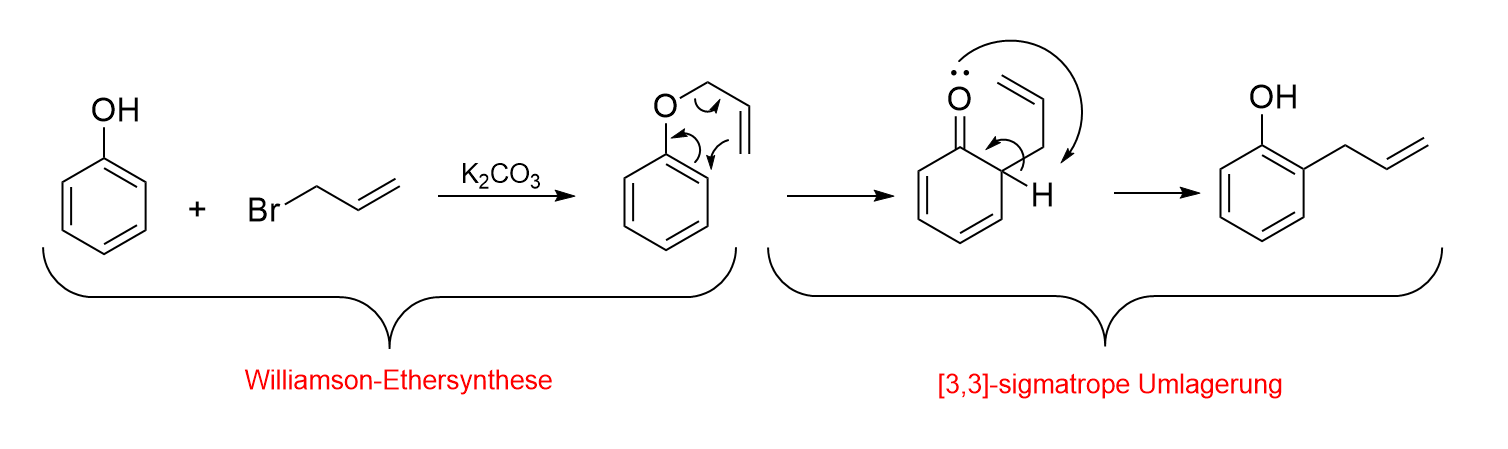
\includegraphics[width=\linewidth]{Bilder/Claisen-Umlagerung.png}
\end{figure}

\subsubsection{Reaktion von Aminen zu Isonitrilen}
\begin{figure}[H]
	\centering
	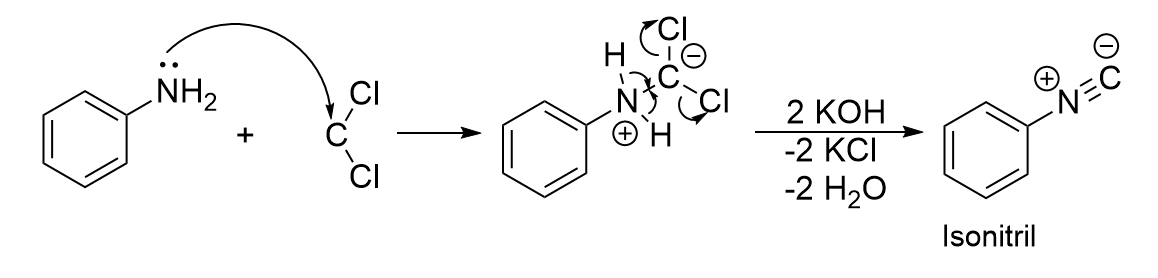
\includegraphics[width=0.8\linewidth]{Bilder/Amine zu Isonitrilen.png}
\end{figure}







\end{document}
